% 若编译失败,且生成 .synctex(busy) 辅助文件,可能有两个原因:
% 1. 需要插入的图片不存在:Ctrl + F 搜索 'figure' 将这些代码注释/删除掉即可
% 2. 路径/文件名含中文或空格:更改路径/文件名即可

% --------------------- 文章宏包及相关设置 --------------------- %
% >> ------------------ 文章宏包及相关设置 ------------------ << %
% 设定文章类型与编码格式
\documentclass[UTF8]{report}		

% 本文特殊宏定义
\def\Re{\mathrm{\,Re}\,}
\def\Im{\mathrm{\,Im}\,}
\def\sinc{\mathrm{\,sinc}\,}
\def\Jc{\mathrm{\,Jc}}


% 自定义宏定义
    \def\N{\mathbb{N}}
    \def\F{\mathbb{F}}
    \def\Z{\mathbb{Z}}
    \def\Q{\mathbb{Q}}
    \def\R{\mathbb{R}}
    \def\C{\mathbb{C}}
    \def\T{\mathbb{T}}
    \def\S{\mathbb{S}}
    \def\A{\mathbb{A}}
    \def\I{\mathscr{I}}
    \def\Im{\mathrm{Im\,}}
    \def\Re{\mathrm{Re\,}}
    \def\d{\mathrm{d}}
    \def\p{\partial}

% 导入基本宏包
    \usepackage[UTF8]{ctex}     % 设置文档为中文语言
        \usepackage{hyperref}  % 宏包:自动生成超链接 (此宏包与标题中的数学环境冲突)
    \hypersetup{
        colorlinks=true,    % false:边框链接 ; true:彩色链接
        citecolor={blue},    % 文献引用颜色
        linkcolor={blue},   % 目录 (我们在目录处单独设置),公式,图表,脚注等内部链接颜色
        urlcolor={magenta},    % 网页 URL 链接颜色,包括 \href 中的 text
        % cyan 浅蓝色 
        % magenta 洋红色
        % yellow 黄色
        % black 黑色
        % white 白色
        % red 红色
        % green 绿色
        % blue 蓝色
        % gray 灰色
        % darkgray 深灰色
        % lightgray 浅灰色
        % brown 棕色
        % lime 石灰色
        % olive 橄榄色
        % orange 橙色
        % pink 粉红色
        % purple 紫色
        % teal 蓝绿色
        % violet 紫罗兰色
    }
    % \usepackage{docmute}    % 宏包:子文件导入时自动去除导言区,用于主/子文件的写作方式,\include{./51单片机笔记}即可。注:启用此宏包会导致.tex文件capacity受限。
    \usepackage{amsmath}    % 宏包:数学公式
    \usepackage{mathrsfs}   % 宏包:提供更多数学符号
    \usepackage{amssymb}    % 宏包:提供更多数学符号
    \usepackage{pifont}     % 宏包:提供了特殊符号和字体
    \usepackage{extarrows}  % 宏包:更多箭头符号
    \usepackage{multicol}   % 宏包:支持多栏 


% 文章页面margin设置
    \usepackage[a4paper]{geometry}
        \geometry{top=1in}
        \geometry{bottom=1in}
        \geometry{left=0.75in}
        \geometry{right=0.75in}   % 设置上下左右页边距
        \geometry{marginparwidth=1.75cm}    % 设置边注距离(注释、标记等)

% 配置数学环境
    %\everymath{\displaystyle}   % 设置全文数学公式都为展示样式
    \usepackage{amsthm} % 宏包:数学环境配置
    % theorem-line 环境自定义
        \newtheoremstyle{MyLineTheoremStyle}% <name>
            {11pt}% <space above>
            {11pt}% <space below>
            {\kaishu}% <body font> 使用默认正文字体
            {}% <indent amount>
            {\bfseries}% <theorem head font> 设置标题项为加粗
            {:}% <punctuation after theorem head>
            {.5em}% <space after theorem head>
            {\textbf{#1}\thmnumber{#2}\ \ (\,\textbf{#3}\,)}% 设置标题内容顺序
        \theoremstyle{MyLineTheoremStyle} % 应用自定义的定理样式
        \newtheorem{LineTheorem}{Theorem.\,}
    % theorem-block 环境自定义
        \newtheoremstyle{MyBlockTheoremStyle}% <name>
            {11pt}% <space above>
            {11pt}% <space below>
            {\kaishu}% <body font> 使用默认正文字体
            {}% <indent amount>
            {\bfseries}% <theorem head font> 设置标题项为加粗
            {:\\ \indent}% <punctuation after theorem head>
            {.5em}% <space after theorem head>
            {\textbf{#1}\thmnumber{#2}\ \ (\,\textbf{#3}\,)}% 设置标题内容顺序
        \theoremstyle{MyBlockTheoremStyle} % 应用自定义的定理样式
        \newtheorem{BlockTheorem}[LineTheorem]{Theorem.\,} % 使用 LineTheorem 的计数器
    % definition 环境自定义
        \newtheoremstyle{MySubsubsectionStyle}% <name>
            {11pt}% <space above>
            {11pt}% <space below>
            {}% <body font> 使用默认正文字体
            {}% <indent amount>
            {\bfseries}% <theorem head font> 设置标题项为加粗
            {:\\ \indent}% <punctuation after theorem head>
            {0pt}% <space after theorem head>
            {\textbf{#3}}% 设置标题内容顺序
        \theoremstyle{MySubsubsectionStyle} % 应用自定义的定理样式
        \newtheorem{definition}{}

%宏包:有色文本框(proof环境)及其设置
    \usepackage[dvipsnames,svgnames]{xcolor}    %设置插入的文本框颜色
    \usepackage[strict]{changepage}     % 提供一个 adjustwidth 环境
    \usepackage{framed}     % 实现方框效果
        \definecolor{graybox_color}{rgb}{0.95,0.95,0.96} % 文本框颜色。修改此行中的 rgb 数值即可改变方框纹颜色,具体颜色的rgb数值可以在网站https://colordrop.io/ 中获得。(截止目前的尝试还没有成功过,感觉单位不一样)(找到喜欢的颜色,点击下方的小眼睛,找到rgb值,复制修改即可)
        \newenvironment{graybox}{%
        \def\FrameCommand{%
        \hspace{1pt}%
        {\color{gray}\small \vrule width 2pt}%
        {\color{graybox_color}\vrule width 4pt}%
        \colorbox{graybox_color}%
        }%
        \MakeFramed{\advance\hsize-\width\FrameRestore}%
        \noindent\hspace{-4.55pt}% disable indenting first paragraph
        \begin{adjustwidth}{}{7pt}%
        \vspace{2pt}\vspace{2pt}%
        }
        {%
        \vspace{2pt}\end{adjustwidth}\endMakeFramed%
        }

% 外源代码插入设置
    % matlab 代码插入设置
    \usepackage{matlab-prettifier}
        \lstset{style=Matlab-editor}    % 继承 matlab 代码高亮 , 此行不能删去
    \usepackage[most]{tcolorbox} % 引入tcolorbox包 
    \usepackage{listings} % 引入listings包
        \tcbuselibrary{listings, skins, breakable}
        \newfontfamily\codefont{Consolas} % 定义需要的 codefont 字体
        \lstdefinestyle{MatlabStyle_inc}{   % 插入代码的样式
            language=Matlab,
            basicstyle=\small\ttfamily\codefont,    % ttfamily 确保等宽 
            breakatwhitespace=false,
            breaklines=true,
            captionpos=b,
            keepspaces=true,
            numbers=left,
            numbersep=15pt,
            showspaces=false,
            showstringspaces=false,
            showtabs=false,
            tabsize=2,
            xleftmargin=15pt,   % 左边距
            %frame=single, % single 为包围式单线框
            frame=shadowbox,    % shadowbox 为带阴影包围式单线框效果
            %escapeinside=``,   % 允许在代码块中使用 LaTeX 命令 (此行无用)
            %frameround=tttt,    % tttt 表示四个角都是圆角
            framextopmargin=0pt,    % 边框上边距
            framexbottommargin=0pt, % 边框下边距
            framexleftmargin=5pt,   % 边框左边距
            framexrightmargin=5pt,  % 边框右边距
            rulesepcolor=\color{red!20!green!20!blue!20}, % 阴影框颜色设置
            %backgroundcolor=\color{blue!10}, % 背景颜色
        }
        \lstdefinestyle{MatlabStyle_src}{   % 插入代码的样式
            language=Matlab,
            basicstyle=\small\ttfamily\codefont,    % ttfamily 确保等宽 
            breakatwhitespace=false,
            breaklines=true,
            captionpos=b,
            keepspaces=true,
            numbers=left,
            numbersep=15pt,
            showspaces=false,
            showstringspaces=false,
            showtabs=false,
            tabsize=2,
        }
        \newtcblisting{matlablisting}{
            %arc=2pt,        % 圆角半径
            % 调整代码在 listing 中的位置以和引入文件时的格式相同
            top=0pt,
            bottom=0pt,
            left=-5pt,
            right=-5pt,
            listing only,   % 此句不能删去
            listing style=MatlabStyle_src,
            breakable,
            colback=white,   % 选一个合适的颜色
            colframe=black!0,   % 感叹号后跟不透明度 (为 0 时完全透明)
        }
        \lstset{
            style=MatlabStyle_inc,
        }

% table 支持
    \usepackage{booktabs}   % 宏包:三线表
    \usepackage{tabularray} % 宏包:表格排版
    \usepackage{longtable}  % 宏包:长表格

% figure 设置
    \usepackage{graphicx}  % 支持 jpg, png, eps, pdf 图片 
    \usepackage{subcaption} % 支持子图
    \usepackage{svg}       % 支持 svg 图片
        \svgsetup{
            % 指向 inkscape.exe 的路径
            inkscapeexe = C:/aa_MySame/inkscape/bin/inkscape.exe, 
            % 一定程度上修复导入后图片文字溢出几何图形的问题
            inkscapelatex = false                 
        }

% 图表进阶设置
    \usepackage{caption}    % 图注、表注
        \captionsetup[figure]{name=图}  
        \captionsetup[table]{name=表}
        \captionsetup{
            labelfont=bf, % 设置标签为粗体
            textfont=bf,  % 设置文本为粗体
            font=small  
        }
    \usepackage{float}     % 图表位置浮动设置 
    \usepackage{etoolbox} % 用于保证图注表注的数学字符为粗体
        \AtBeginEnvironment{figure}{\boldmath} % 图注中的数学字符为粗体
        \AtBeginEnvironment{table}{\boldmath}  % 表注中的数学字符为粗体
        \AtBeginEnvironment{tabular}{\unboldmath}   % 保证表格中的数学字符不受额外影响

% 圆圈序号自定义
    \newcommand*\circled[1]{\tikz[baseline=(char.base)]{\node[shape=circle,draw,inner sep=0.8pt, line width = 0.03em] (char) {\small \bfseries #1};}}   % TikZ solution

% 列表设置
\usepackage{enumitem}   % 宏包:列表环境设置
    \setlist[enumerate]{
        label=\bfseries(\arabic*) ,   % 设置序号样式为加粗的 (1) (2) (3)
        ref=\arabic*, % 如果需要引用列表项,这将决定引用格式(这里仍然使用数字)
        itemsep=0pt, parsep=0pt, topsep=0pt, partopsep=0pt, leftmargin=3.5em} 
    \setlist[itemize]{itemsep=0pt, parsep=0pt, topsep=0pt, partopsep=0pt, leftmargin=3.5em}
    \newlist{circledenum}{enumerate}{1} % 创建一个新的枚举环境  
    \setlist[circledenum,1]{  
        label=\protect\circled{\arabic*}, % 使用 \arabic* 来获取当前枚举计数器的值,并用 \circled 包装它  
        ref=\arabic*, % 如果需要引用列表项,这将决定引用格式(这里仍然使用数字)
        itemsep=0pt, parsep=0pt, topsep=0pt, partopsep=0pt, leftmargin=3.5em
    }  
    

% 其它设置
    % 脚注设置
    \renewcommand\thefootnote{\ding{\numexpr171+\value{footnote}}}
    % 参考文献引用设置
        \bibliographystyle{unsrt}   % 设置参考文献引用格式为unsrt
        \newcommand{\upcite}[1]{\textsuperscript{\cite{#1}}}     % 自定义上角标式引用
    % 文章序言设置
        \newcommand{\cnabstractname}{序言}
        \newenvironment{cnabstract}{%
            \par\Large
            \noindent\mbox{}\hfill{\bfseries \cnabstractname}\hfill\mbox{}\par
            \vskip 2.5ex
            }{\par\vskip 2.5ex}

% 文章默认字体设置
    \usepackage{fontspec}   % 宏包:字体设置
        \setmainfont{SimSun}    % 设置中文字体为宋体字体
        \setCJKmainfont[AutoFakeBold=3]{SimSun} % 设置加粗字体为 SimSun 族,AutoFakeBold 可以调整字体粗细
        \setmainfont{Times New Roman} % 设置英文字体为Times New Roman

% 各级标题自定义设置
    \usepackage{titlesec}   
    % chapter
        \titleformat{\chapter}[hang]{\normalfont\Large\bfseries\centering\boldmath}{Homework \thechapter :}{10pt}{}
        \titlespacing*{\chapter}{0pt}{-30pt}{10pt} % 控制上方空白的大小
    % section
        \titleformat{\section}[hang]{\normalfont\large\bfseries\boldmath}{\thesection}{8pt}{}
    % subsection
        % 设置 subsection 样式为 (1) (2) (3)
        \renewcommand{\thesubsection}{(\arabic{subsection})}    
        \titleformat{\subsection}[hang]{\normalfont\bfseries\boldmath}{\thesubsection}{8pt}{}    

% --------------------- 文章宏包及相关设置 --------------------- %
% >> ------------------ 文章宏包及相关设置 ------------------ << %



% ------------------------ 文章信息区 ------------------------ %
% >> --------------------- 文章信息区 --------------------- << %
% 页眉页脚设置

\usepackage{fancyhdr}   %宏包:页眉页脚设置
    \pagestyle{fancy}
    \fancyhf{}
    \cfoot{\thepage}
    \renewcommand\headrulewidth{1pt}
    \renewcommand\footrulewidth{0pt}
    \chead{光学课程作业,\ 丁毅,\ 2023K8009908031}
    \lhead{Homework \thechapter}
    \rhead{\small dingyi233@mails.ucas.ac.cn}

%文档信息设置
\title{光学课程作业\\ Homework of Optics}
\author{丁毅\\ \footnotesize 中国科学院大学,北京 100049\\ Yi Ding \\ \footnotesize University of Chinese Academy of Sciences, Beijing 100049, China}
\date{\footnotesize 2024.9 -- 2025.1}
% >> --------------------- 文章信息区 --------------------- << %
% ------------------------ 文章信息区 ------------------------ %

% 开始编辑文章

\begin{document}
\zihao{5}           % 设置全文字号大小

% ------------------------ 封面序言与目录 ------------------------ %
% >> --------------------- 封面序言与目录 --------------------- << %
% 封面
    \maketitle\newpage  
    \pagenumbering{Roman} % 页码为大写罗马数字
    \thispagestyle{fancy}   % 显示页码、页眉等

% 序言
    \begin{cnabstract}\normalsize 
        本文为笔者本科时的“光学”课程作业(Homework of Optics, 2024.9-2025.1)。本门课程笔记和其他科目的笔记、作业,例如热学、电磁学、电路原理和数学物理方法等,也可以在我的 \href{https://github.com/YiDingg/LatexNotes}{GitHub > LatexNotes} 仓库上找到。

        每次提交作业,老师给予批阅反馈之后,会对原作业内容进行修改、订正,以期达到满分作业的参考标准。但是,由于个人学识浅陋,认识有限,文中难免有不妥甚至错误之处,望读者不吝指正。读者可以将错误发送到我的邮箱 {\color{blue}\ dingyi233@mails.ucas.ac.cn},也可以到笔者的 \href{https://github.com/YiDingg/LatexNotes}{GitHub (https://github.com/YiDingg/LatexNotes)} 上提 \href{https://github.com/YiDingg/LatexNotes/issues}{issue},衷心感谢。
    \end{cnabstract}
    \addcontentsline{toc}{chapter}{序言} % 手动添加为目录

% 不换页目录
    \setcounter{tocdepth}{0}
    \noindent\rule{\textwidth}{0.1em}   % 分割线
    \noindent\begin{minipage}{\textwidth}\centering 
        \vspace{1cm}
        \tableofcontents\thispagestyle{fancy}   % 显示页码、页眉等   
    \end{minipage}  
    \addcontentsline{toc}{chapter}{目录} % 手动添加为目录

% 收尾工作
    \newpage    
    \pagenumbering{arabic} 

% >> --------------------- 封面序言与目录 --------------------- << %
% ------------------------ 封面序言与目录 ------------------------ %

\chapter{第一章作业}\thispagestyle{fancy}

\section{求入射到光纤的角度满足的条件}
\begin{equation}
    n_0 \sin i = n_g \sin i', \quad n_g \sin (\frac{\pi}{2} - i') = n_c \sin \frac{\pi}{2} 
     \Longrightarrow i \leqslant \arcsin \left( \frac{n_g}{n_0} \sqrt{1 - \frac{n_c^2}{n_g^2}}\,  \right)
\end{equation}
    

\begin{figure}[H]\centering
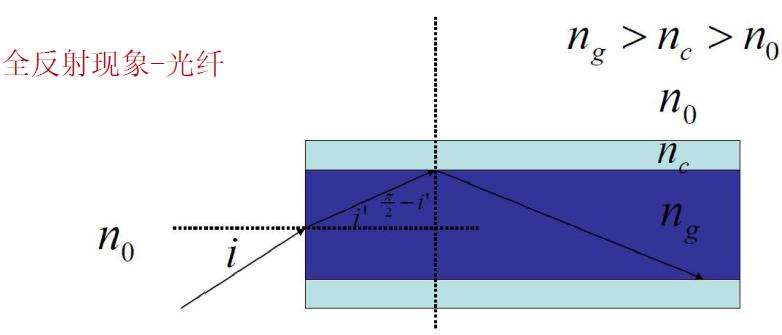
\includegraphics[width=0.55\textwidth]{assets/1/c6c9e6ef2f6755ead534508010ad0452 (2).jpg}
\caption{\textbf{求入射到光纤的角度满足的条件}}\label{求入射到光纤的角度满足的条件}
\end{figure}

\section{推导光线轨迹方程}

在 $x$-$y$ 平面中,设 $y = y(x)$ 表示光线的轨迹方程,$n = n(y)$ 表示介质的折射率。由几何关系,我们有:
\begin{equation}
\frac{\mathrm{d} y }{\mathrm{d} x } = \tan \theta = \frac{1}{\tan i} = \frac{\sqrt{1-\sin^2 i}}{\sin i} 
\end{equation}

由折射定律,记 $[n(y)\sin i(y)]_{y=0} = C$ ,则我们有:
\begin{equation}
n(y)\sin i(y) = C  \Longrightarrow \frac{\mathrm{d} y }{\mathrm{d} x } = \frac{\sqrt{n^2 - C^2}}{C^2}, \quad \left(\frac{\mathrm{d} y }{\mathrm{d} x }\right)^{2} = \frac{n^2}{C^2} - 1
\end{equation}
两边同时对 $x$ 求导,得到:
\begin{equation}
2 \left(\frac{\mathrm{d} y }{\mathrm{d} x }\right) \left(\frac{\mathrm{d}^2 y }{\mathrm{d} x^2 }\right) = \frac{1}{C^2} \left(\frac{\mathrm{d} n^2 }{\mathrm{d} y }\right) \left(\frac{\mathrm{d} y }{\mathrm{d} x }\right) \Longrightarrow \frac{\mathrm{d}^2 y }{\mathrm{d} x^2 } = \frac{1}{2C^2}\cdot \frac{\mathrm{d} n^2 }{\mathrm{d} y } 
\end{equation}
也即
\begin{equation}
    \frac{\mathrm{d}^2 y }{\mathrm{d} x^2 } = \frac{1}{2n_0^2\sin^2 i_0}\cdot \frac{\mathrm{d} n^2 }{\mathrm{d} y } = \frac{1}{2n_0^2\cos^2 \theta_0}\cdot \frac{\mathrm{d} n^2 }{\mathrm{d} y } \quad \square
\end{equation}

\begin{figure}[H]\centering
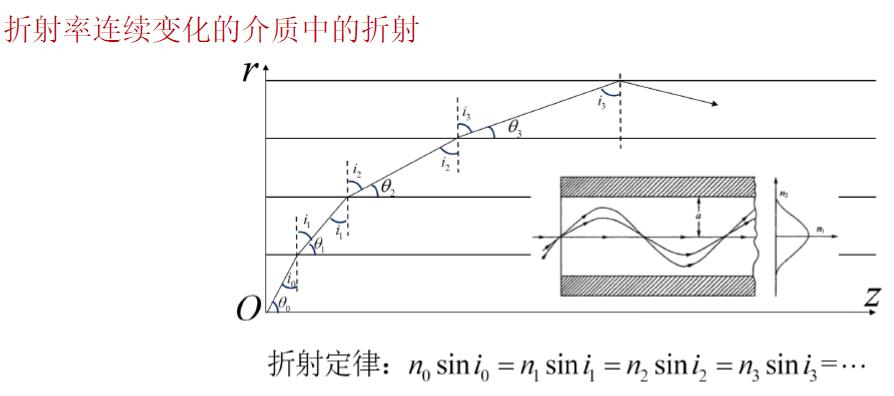
\includegraphics[width=0.8\textwidth]{assets/1/88b3f41951f9d3be9e2964935ebaf0f7.jpg}
\caption{\textbf{推导光线轨迹方程}}\label{推导光线轨迹方程}
\end{figure}

事实上,在三维坐标系中考虑上述过程,或者利用费马原理和变分法,又或考虑哈密顿光学,可以得到更一般的形式,称为光路方程,如下:
\begin{equation}
    \nabla n=\frac{\mathrm{d}}{\mathrm{d}s}\left(n\frac{\mathrm{d}\vec{r}}{\mathrm{d}s}\,\right)
\end{equation}

\section{(已被删去)}
\section{利用费马原理给出物像关系}

折射球面如图,由余弦定理可知:
\begin{equation}
\text{OPL} = np + n'p' 
= n \sqrt{r^2 + (s+r)^2 \,{\color{red} -}\, 2r(s+r)\cos \phi } + n' \sqrt{r^2 + (s'-r)^2 \,{\color{red} +}\, 2r(s'-r)\cos \phi } 
\end{equation}

由费马原理,$\frac{\mathrm{d} \text{OPL}  }{\mathrm{d} \phi } = 0$,于是:
\begin{equation}
\frac{-nr(s+r)\sin \phi }{p} + \frac{n'r(s'-r)\sin \phi }{p'} = 0 \Longrightarrow  \frac{n}{p} + \frac{n'}{p'} = \frac{1}{R\,}\left( \frac{n's'}{p'} - \frac{ns}{p} \right)
\end{equation}

在傍轴条件下,有 $s \approx p$,$s' \approx p'$,于是:
\begin{equation}
\frac{n}{s} + \frac{n'}{s'} = \frac{n' - n}{R}   \quad\square
\end{equation}
证毕。
\begin{figure}[H]\centering
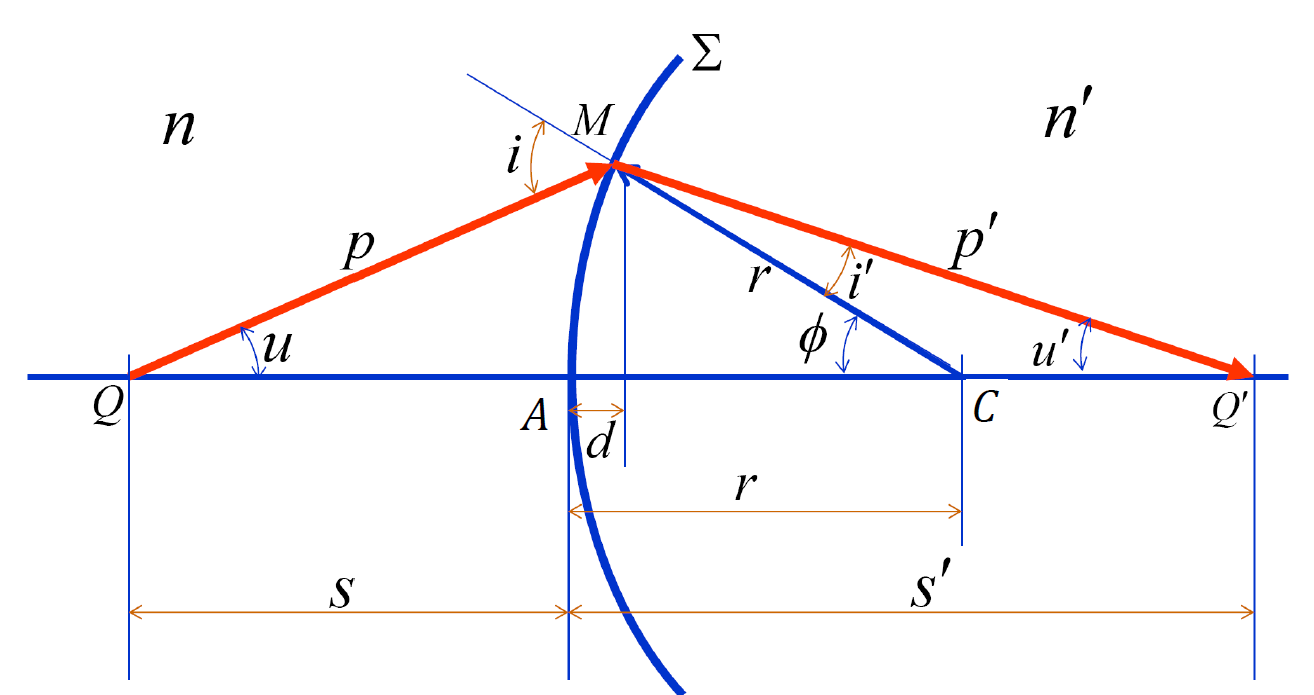
\includegraphics[width=0.45\textwidth]{assets/1/7dd67844c3c8000268c32546583de193.png}
\caption{\textbf{折射球面物像关系}}\label{折射球面物像关系}
\end{figure}

\section{推导反射球面的物像公式}

这里要注意,由于像是虚像,$l_2$ 贡献虚光程(为负),且 $s_2<0$,因此圆心到像点的距离为 $r+s_2$ 而非 $r-s_2$。同由余弦定理,写出光程 \text{OPL},有:
\begin{equation}
\text{OPL} = n_1l_1 - n_2l_2 
=
n_1\sqrt{r^2 + (r+s_1)^2 - 2r(r+s_1)\cos \phi } \,{\color{red} -}\, n_2 \sqrt{r^2 + (r+s_2)^2 - 2r(r+s_2)\cos \phi } 
\end{equation}

由费马原理,$\frac{\mathrm{d} \text{OPL}  }{\mathrm{d} \phi } = 0$,于是有:
\begin{equation}
\frac{-n_1r(r+s_1)\sin \phi }{l_1} + \frac{n_2r(r+s_2)\sin \phi }{l_2} = 0 
\Longrightarrow 
\frac{n_2}{l_2} - \frac{n_1}{l_1} = \frac{1}{r}\left( \frac{n_1s_1}{l_1} - \frac{n_2s_2}{l_2} \right)
\end{equation}
傍轴时,有 $s_1 \approx l_1$,$s_2 \approx -l_2$,于是:
\begin{equation}
-\frac{n_2}{l_2} - \frac{n_1}{l_1} = \frac{1}{r}(n_1 + n_2)
\end{equation}
当反射球面两侧为相同介质时,$n_1 = n_2$,则:
\begin{equation}
\frac{1}{s_1} + \frac{1}{s_2} = -\frac{2}{r}  \quad\square
\end{equation}
证毕。

\section{画出图中的像点}
如下图所示,左侧为手绘图,右侧为光路仿真软件 \href{https://www.optico.app/en/start-en/}{Optico} 效果图。

\begin{figure}[H]\centering
\begin{subfigure}[t]{0.47\textwidth}\centering
    \includegraphics[height=130pt]{assets/1/图1.png}
    \caption{ 手绘图 }
\end{subfigure}\begin{subfigure}[t]{0.52\textwidth}\centering
    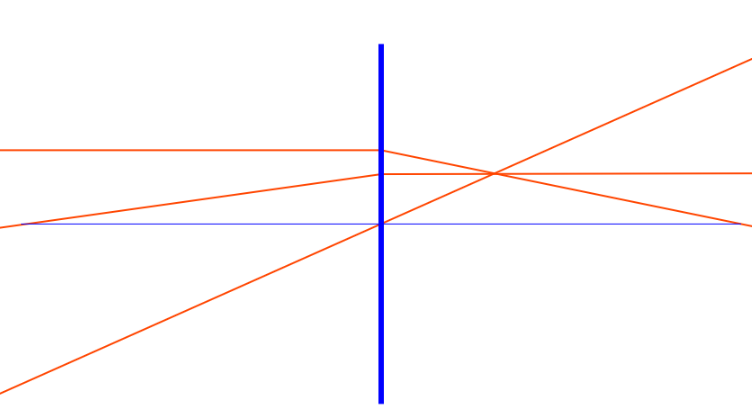
\includegraphics[height=130pt]{assets/1/1.png}
    \caption{ 光路仿真 }
\end{subfigure}
\caption{ 画出虚物 $Q$ 的像点 $Q'$}
\end{figure}

\begin{figure}[H]\centering
    \begin{subfigure}[t]{0.47\textwidth}\centering
        \includegraphics[height=130pt]{assets/1/图2.png}
        \caption{ 手绘图 }
    \end{subfigure}\begin{subfigure}[t]{0.52\textwidth}\centering
        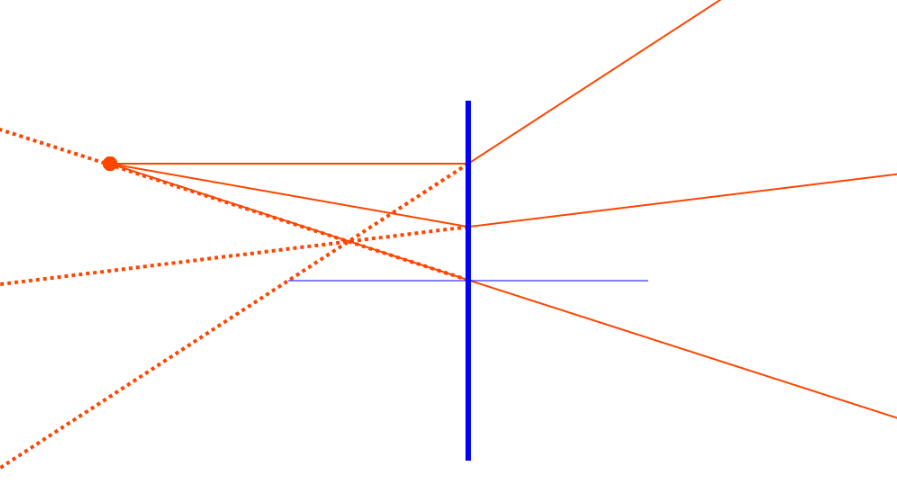
\includegraphics[height=130pt]{assets/1/2.png}
        \caption{ 光路仿真 }
    \end{subfigure}
    \caption{ 画出实物 $Q$ 经凹透镜的像点 $Q'$}
\end{figure}

    \begin{figure}[H]\centering
\begin{subfigure}[t]{0.47\textwidth}\centering
    \includegraphics[height=130pt]{assets/1/图3.png}
    \caption{ 手绘图 }
\end{subfigure}\begin{subfigure}[t]{0.52\textwidth}\centering
    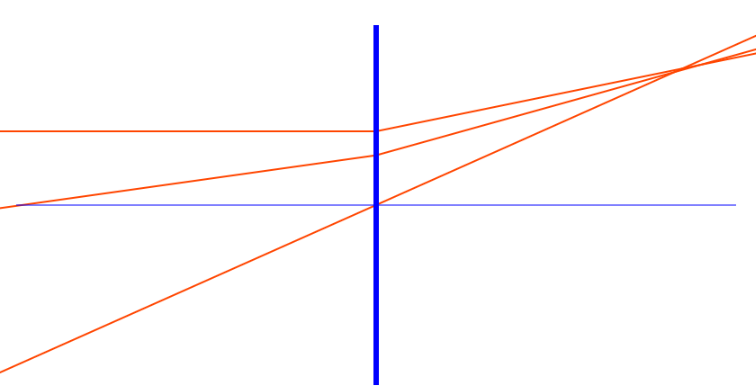
\includegraphics[height=130pt]{assets/1/3.png}
    \caption{ 光路仿真 }
\end{subfigure}
\caption{ 画出虚物 $Q$ 经凹透镜的像点 $Q'$}
\end{figure}



\chapter{第二章作业}\thispagestyle{fancy}
\vspace{-2mm}
\section{对于正入射的情况,写出菲涅尔公式}

菲涅尔公式如下:

\begin{table}[H]
    \centering
    \renewcommand{\arraystretch}{1.5} % 调整行间距为默认值的1.5倍 
    \begin{tabular}{|c|c|c|c|c|} 
    \hline
    类型 & \multicolumn{2}{c|}{振幅反射系数 $r$} & \multicolumn{2}{c|}{振幅透射系数 $t$ }  \\ 
    \hline
    s 波 & $\displaystyle r_s = \frac{n_i\cos \theta_i - n_t \cos \theta_t}{n_i\cos \theta_i + n_t \cos \theta_t} $ & $\displaystyle  - \frac{\sin (\theta_i - \theta_t) }{\sin (\theta_i + \theta_t)}$ & $\displaystyle t_s  = \frac{2n_i \cos \theta_i}{n_i\cos \theta_i + n_t \cos \theta_t} $ &   $\displaystyle  + \frac{2 \sin \theta_t \cos \theta_i}{\sin (\theta_i + \theta_t)}$   \\ 
    \hline
    p 波 & $\displaystyle r_p = \frac{n_t\cos \theta_i - n_i \cos \theta_t}{n_t\cos \theta_i + n_i \cos \theta_t} $ &     $ \displaystyle  + \frac{\tan (\theta_i - \theta_t)}{\tan (\theta_i + \theta_t)} $  &  $\displaystyle t_p  = \frac{2n_i \cos \theta_i}{n_i\cos \theta_t + n_t \cos \theta_i} $ &   $\displaystyle + \frac{2 \sin \theta_t \cos \theta_i}{\sin (\theta_i + \theta_t) \cos (\theta_i - \theta_t)}$                  \\
    \hline
    \end{tabular}
\end{table}

正入射时,$\theta_i = \theta_t = 0$,于是有:
\begin{gather}
    r_p = (-r_s)  = \frac{n_t - n_i}{n_t + n_i},\quad t_p = t_s = \frac{2n_i}{n_i + n_t} \\ 
    F = R_s = R_p = \left( \frac{n_t - n_i}{n_t + n_i} \right)^2
\end{gather}


不妨作出相关的图像,图 \ref{振幅系数随入射角的变化} 是 s 波、p 波振幅系数关于入射角 $\theta_i$ 的变化情况\footnote{源码见附录 \ref{图振幅系数随入射角的变化源码}}。

\begin{figure}[H]\centering
\begin{subfigure}[t]{0.49\textwidth}\centering
    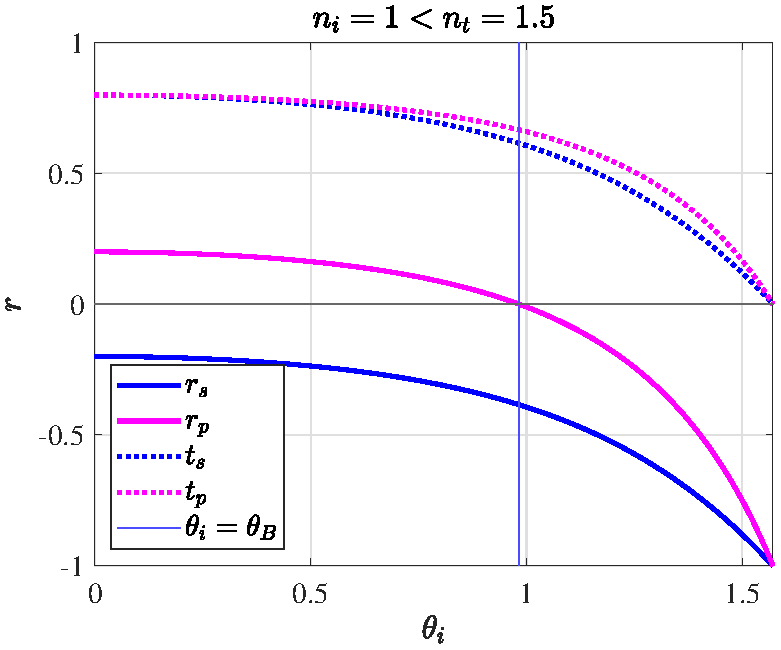
\includegraphics[height=180pt]{assets/2/2024-09-15_10-53-31.pdf}
    \caption{ 由空气入射玻璃($n_i = 1,\ n_t = 1.5$) }
\end{subfigure}
\begin{subfigure}[t]{0.49\textwidth}\centering
    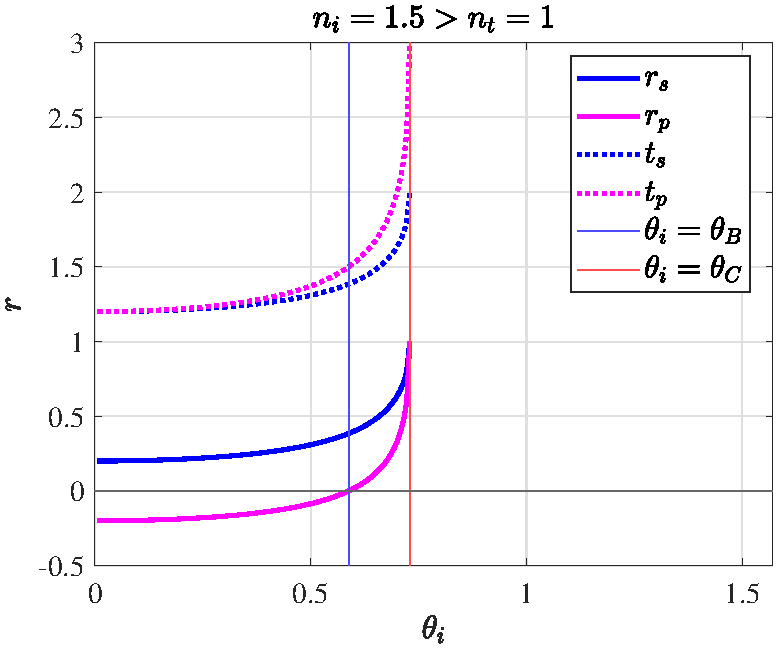
\includegraphics[height=180pt]{assets/2/2024-09-15_10-53-27.pdf}
    \caption{ 由玻璃入射空气($n_i = 1.5,\ n_t = 1$) }
\end{subfigure}
\caption{ 振幅系数 $r$ 随入射角 $\theta_i$ 的变化 }\label{振幅系数随入射角的变化}
\end{figure}

\vspace{-7mm}
\section{一自然光以 Brewster Angle 入射到空气中的一块玻璃,已知功率透射率为 0.86。}

%{\color{red} $\star $ 事实上,本题题设并不合理,是不符合实际的。我们先给出解题过程,再说明为何玻璃折射率。}

\textbf{(1)\ \ 求功率的反射率}

$T = 0.86$,由能量守恒,功率反射率 $R = 0.14$。

\textbf{(2)\ \ 若输入为 1000 W,求透射光 s 分量上的功率}

光束为自然光,因此 s 分量和 p 分量的功率相同,都为 500 W,也即 $\Phi_{e,i,s} = \Phi_{e,i,p} = 500 \ \mathrm{W}$。又由 Brewster Angle 入射,因此反射光的 p 分量为 0,也即 $R_p = 0$,于是:
\begin{gather}
T_p = 1 - R_p = 1,\quad T_s = 2T - T_p = 0.72 
\end{gather}
由此可求得透射光 s 分量上的辐射通量(即辐射功率):
\begin{equation}
\Phi_{e,t,s} = T_s \Phi_{e,i,s} = 0.72 \times 500 \ \mathrm{W} =  360 \ \mathrm{W}
\end{equation}

{\color{red} \textbf{(3)\ \ 求玻璃的折射率}}

虽然题目并未要求\footnote{查阅资料发现,此题来自于\textit{光学(尤金,第五版)Optics (Eugene Hecht)} 的 Page 152},但我们不妨求解一下玻璃的折射率 $n_t$。在题设条件下,$R = 0.14$,默认空气折射率为 1,则唯一的未知量是玻璃折射率 $n_t$,这是可以求解的,方程如下:
\begin{gather}\label{玻璃折射率}
    R = \frac{1}{2}(R_s + R_p) = 0.14,\quad \theta_i = \theta_B = \arctan\left(\frac{n_t}{n_i}\right) ,\quad n_i = 1
    \Longrightarrow \\ 
    \left[ \frac{ \cos (\arctan n_t) - \sqrt{n_{t}^2 - \sin^2 (\arctan n_t)} }{\cos (\arctan n_t) + \sqrt{n_{t}^2 - \sin^2 (\arctan n_t)}} \right]^2 + \left[ \frac{ n_{t}^2\cos (\arctan n_t) - \sqrt{n_{t}^2 - \sin^2 (\arctan n_t)} }{n_{t}^2\cos (\arctan n_t) + \sqrt{n_{t}^2 - \sin^2 (\arctan n_t)}} \right]^2  = 2\times 0.14
\end{gather}
此方程有唯一未知量 $n_t$,用 Matlab 解此非线性方程组\footnote{源码见附录 \ref{玻璃折射率源码}},得到玻璃折射率 $n_t$,以及其它参量\footnote{图 \ref{方程左边的变化情况} 源码见附录 \ref{方程左边的变化情况源码}}: 
\begin{gather}
\begin{cases}
    n_t = 0.554902 
    ,\quad 
    \theta_i = \theta_B  = 29.025970^\circ
    \\
    \theta_t = 60.974030^\circ
    ,\quad 
    \theta_C = 33.703947^\circ
    \\
    R = 0.1400,\quad   R_s = 0.280000,\    R_p = 0.000000 \\ 
    T = 0.8600,\quad   T_s = 0.720000,\    T_p = 1.000000 
\end{cases}
\begin{cases}
    n_t = 1.802121
    ,\quad 
    \theta_i = \theta_B  = 60.974030^\circ 
    \\
    \theta_t = 29.025970^\circ
    ,\quad 
    \theta_C = 90.000000^\circ
    \\
    R = 0.1400,\quad   R_s = 0.280000,\    R_p = 0.000000 \\ 
    T = 0.8600,\quad   T_s = 0.720000,\    T_p = 1.000000 
\end{cases}
\end{gather}



\begin{center}\noindent\begin{minipage}{0.50\textwidth}
\hspace*{2em} 也即上述方程有两解,考虑 $n_{ti} \in [0,\ 2]$,令方程左边为 $f(n_{ti})$,作出图像如右。图 \ref{方程左边的变化情况} 说明了我们并没有漏掉其它解。

\hspace*{2em} 一般玻璃的折射率在 1.5 左右,即使是特殊玻璃(例如高折射率镜片),也基本在 1.3 至 1.9 之间,0.5 的玻璃折射率显然是不合理的,即使是考虑介质折射率关于波长的变化(如 X 射线或 Gamma 射线),也不会达到如此低的折射率。因此舍去 $n_t = 0.554902$,最终得 $n_t = 1.802121$。
\end{minipage}\hfill\begin{minipage}{0.43\textwidth}
    \begin{figure}[H]\centering
        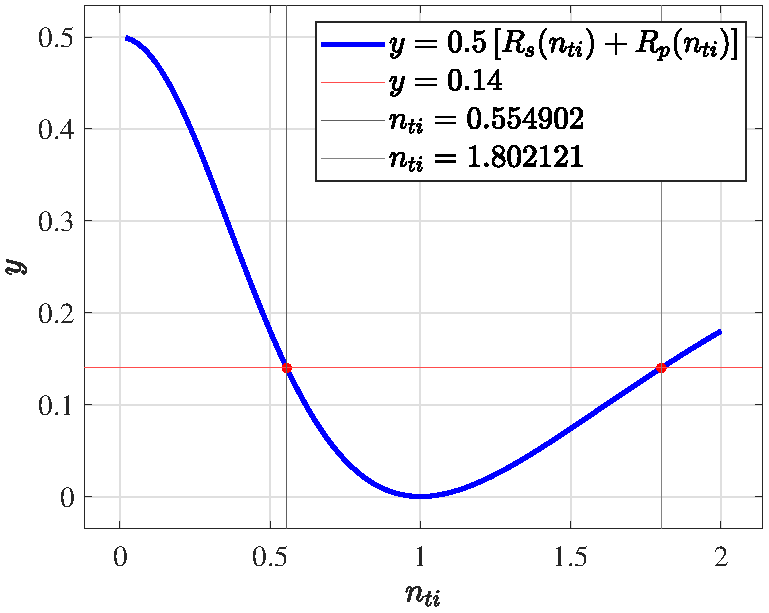
\includegraphics[width=\textwidth]{assets/2/2024-09-18_01-08-40.pdf}
        \vspace*{-9mm}
        \caption{ 方程 \ref{玻璃折射率} 左边函数值随 $n_{ti}$ 的变化情况}\label{方程左边的变化情况}
        \end{figure}
\end{minipage}\end{center}



\section*{上题改编:一自然光由空气入射玻璃,玻璃折射率为 1.5,已知功率透射率为 0.86。}


\textbf{(1)\ \ 求功率的反射率:}

$T = 0.86$,由能量守恒,功率反射率 $R = 0.14$。

\textbf{(2)\ \ 若输入为 1000 W,求透射光 s 分量上的功率}

光束为自然光,因此 s 分量和 p 分量的功率相同,都为 500 W。先求解入射角 $\theta_i$,由菲涅尔定理和能量关系:
\begin{equation}
R =  \frac{1}{2}(R_s + R_p),\  R_s =  \left[ \frac{ \cos \theta_i - \sqrt{n_{ti}^2 - \sin^2 \theta_i} }{\cos \theta_i + \sqrt{n_{ti}^2 - \sin^2 \theta_i}} \right]^2,\ R_p = \left[ \frac{ n_{ti}^2\cos \theta_i - \sqrt{n_{ti}^2 - \sin^2 \theta_i} }{n_{ti}^2\cos \theta_i + \sqrt{n_{ti}^2 - \sin^2 \theta_i}} \right]^2
\end{equation}
其中 $n_i = 1$,$n_t = 1.5$,因此 $n_{ti} = 1.5$,代入即得:
\begin{equation}
    \left[ \frac{ \cos \theta_i - \sqrt{1.5^2 - \sin^2 \theta_i} }{\cos \theta_i + \sqrt{1.5^2 - \sin^2 \theta_i}} \right]^2 + \left[ \frac{ 1.5^2\cos \theta_i - \sqrt{1.5^2 - \sin^2 \theta_i} }{1.5^2\cos \theta_i + \sqrt{1.5^2 - \sin^2 \theta_i}} \right]^2 = 2\times0.14
\end{equation}
用 Matlab 解此非线性方程组\footnote{源码见附录 \ref{公式解入射角源码}},得到入射角 $\theta_i$ 和其它参量:
\begin{gather}\label{解入射角}
\begin{matrix}
    \theta_i =  1.173220\ \ \mathrm{rad}  = 67.220559^\circ \\
    R = 0.140000,\quad   R_s = 0.256933,\    R_p = 0.023067 \\ 
    T = 0.860000,\quad   T_s = 0.743067,\    T_p = 0.976933
\end{matrix}
\end{gather}

于是透射光 s 分量上的辐射通量为:
\begin{equation}
\Phi_{e,t,s} = T_s \Phi_{e,i,s} = 0.743067 \times 500 \ \mathrm{W} =  371.5335 \ \mathrm{W}
\end{equation}


\section{光束垂直入射到玻璃-空气界面,玻璃折射率 1.5,求出能量反射率和透射率}

$\theta_i = 0$ 时,由菲涅尔定律和能量关系,有:
\begin{gather}
    R =  \frac{1}{2}(R_s + R_p),\quad  T = 1 - R\\ 
    R_s =  \left[ \frac{ \cos \theta_i - \sqrt{n_{ti}^2 - \sin^2 \theta_i} }{\cos \theta_i + \sqrt{n_{ti}^2 - \sin^2 \theta_i}} \right]^2 = \left[ \frac{1 - n_{ti}}{1 + n_{ti}} \right]^2,\ R_p = \left[ \frac{ n_{ti}^2\cos \theta_i - \sqrt{n_{ti}^2 - \sin^2 \theta_i} }{n_{ti}^2\cos \theta_i + \sqrt{n_{ti}^2 - \sin^2 \theta_i}} \right]^2 =  \left[ \frac{n_{ti}^2 - n_{ti}}{n_{ti}^2 + n_{ti}} \right]^2
\end{gather}
由空气入射玻璃时,$n_{ti} = 1.5$,由玻璃入射空气时,$n_{ti} = \frac{2}{3}$,代入得到:
\begin{gather*}
\text{空气入射玻璃: }\ R = 0.04,\quad  T = 0.96 \\ 
\text{玻璃入射空气: }\ R = 0.04,\quad  T = 0.96 
\end{gather*}
也即无论从哪边入射,能量反射率和透射率分别为 0.04 和 0.96。


\chapter{第三章作业}\thispagestyle{fancy}

\section{在杨氏双缝实验中,设两缝之间的距离为 0.2 mm,在距双缝 1 m 远的屏上观察干涉
条纹,若入射光是波长为 400 nm 至 760 nm 的白光,问屏上距零级明纹 20 mm 处,哪些波
长的光最大限度地加强?}

也即求哪些波长的光在 20 mm 处是亮条纹。杨氏干涉中,两相邻亮(暗)条纹的间距 $\Delta x = \frac{D \lambda}{d}$,其中 $D$ 是双缝屏与屏幕的距离,$d$ 是双缝间距,$\lambda$ 是波长。因此有:
\begin{gather}
k \Delta x = 20 \ \mathrm{mm} \Longrightarrow \lambda = \frac{d\cdot 20 \ \mathrm{mm}}{D} \cdot \frac{1 }{k} = \frac{4}{k}\times 10^{-6},\quad k = 1,2,3,\cdots
\end{gather}
而波长范围 $\lambda \in [400 \ \mathrm{nm} ,\ 760 \ \mathrm{nm}]$,于是:
\begin{equation}
k \in [5.2632,\ 10] \Longrightarrow k = 6,7,8,9,10 ,\quad \lambda = 400.0 \ \mathrm{nm},\ 444.4 \ \mathrm{nm},\ 500.0 \ \mathrm{nm},\ 571.4 \ \mathrm{nm},\ 666.7 \ \mathrm{nm}
\end{equation}

\section{在空气中用某单色光进行双缝干涉实验时,观察到干涉条纹相邻明条纹的间距为
1.33 mm,当把实验装置放在水中时(水的折射率为 1.33),则相邻明条纹的间距变为多
少?}

空气折射率近似为 1,设光在空气中的波长为 $\lambda$,则在水中的波长为 $\frac{\lambda}{n}$,其中 $n$ 为水的折射率。而双缝干涉中相邻亮条纹间距为:
\begin{equation}
\Delta x = \frac{D \lambda}{d} \Longrightarrow \Delta x' = \frac{\Delta x}{n} = 1\ \mathrm{mm}
\end{equation}

\section{用波长为 589.3 nm 的钠黄光垂直照射长 $\boldsymbol{L = 20 \ \mathrm{mm}}$  的空气尖劈,测得条纹间距为 $\boldsymbol{1.18}$ $\boldsymbol{ \times 10^{-4}\ \mathrm{m}}$,求钢球直径 $\boldsymbol{d}$。}

构成劈尖干涉,相邻亮条纹间距为 $\Delta x = \frac{\lambda}{2 \tan \theta} \approx  \frac{\lambda}{2 \theta} $,设劈尖长为 $L$,倾角为 $\theta$,钢球的直径为 $D$,则有:
\begin{equation}
\tan \theta = \frac{D}{L} \Longrightarrow D =  L \tan \theta \approx \theta L  = \frac{\lambda L}{2 \Delta x} = 4.9941 \times 10^{-5}\ \mathrm{m}
\end{equation}
即为所求直径。

\section{厚度为 0.050 mm 的玻璃片,其折射率为 1.520,插入迈克尔孙干涉仪的一条光路中,照明光为波长 587.56 nm 的氦黄线。求插入这片玻璃片移动了多少干涉条纹?}

改变两干涉光束的光程差,会使原干涉条纹发生移动。设 $n_f$ 为玻璃片折射率,$d$ 为玻璃片厚度,$\lambda_0$ 为氦黄线在空气中的波长,则有:
\begin{equation}
2 n_f d = N\lambda_0 \Longrightarrow N = \frac{2 n_f d}{\lambda_0} = 258.6970
\end{equation}

\section{迈克耳逊干涉仪两臂中分别加入 20 cm 长的玻璃管,一个抽成真空,一个充以一个大气压的氩气,今以汞光线(波长为 546.0 nm)入射干涉仪,如将氩气抽出,发现干涉仪
中条纹移动了 205 条,求氩气的折射率。}

抽成真空的玻璃管补偿了穿过玻璃管带来的光程,因此没有引入附加光程差。与上题同理,设 $n_f$ 为氩气折射率,$d$ 为玻璃管长度,$\lambda_0$ 为汞光线在空气中的波长,并近似空气折射率为 1,则有: 
\begin{equation}
2 (n_f-1) d = N\lambda_0 \Longrightarrow n_f = \frac{N \lambda_0}{2d} + 1 = 1.0002798
\end{equation}

\section{有一谱线结构,谱线范围是 500 nm 至 501 nm,若 F-P 标准具 $d = 0.5 \ \mathrm{mm}$,可否用它来分析这一谱线结构?}

波长的自由光谱宽度 $\left(\Delta\lambda\right)_{\text{fsr}}$、最小分辨率 $\left(\Delta\lambda\right)_{\min}$ 和极限分辨率 $\left(\Delta\lambda\right)_{\lim}$ 分别为:
\begin{equation}
    \left(\Delta\lambda\right)_{\text{fsr}} = \frac{\lambda_0^2}{2 n d}
    ,\quad 
    \left(\Delta\lambda\right)_{\min} = \frac{2\lambda_0}{\pi \sqrt{F}}
    ,\quad 
    \left(\Delta\lambda\right)_{\lim} = \frac{\lambda_0^2}{\pi n d \sqrt{F}}
\end{equation}
代入数据 $d = 0.5 \ \mathrm{mm}$,空气折射率近似 $n = 1$,并取能量反射率为典型值 $R = 0.90$,可以得到:
\begin{equation}
F = 80.0000 ,\quad 
\left(\Delta\lambda\right)_{\text{fsr}} = 0.2505 \ \mathrm{nm}
,\quad
\left(\Delta\lambda\right)_{\min} = 0.0011 \ \mathrm{nm}
,\quad 
\left(\Delta\lambda\right)_{\lim} = 5.6382 \times 10^{-7} \ \mathrm{nm}
\end{equation}
而谱线宽度 $\Delta \lambda = 1 \ \mathrm{nm} > \left(\Delta\lambda\right)_{\text{fsr}}$,因此,无论光谱是连续谱还是分立谱,虽然可以观察到明显的干涉条纹(对分立谱),或者在频谱分析仪中看到明显的频率纵模(对连续谱),但是都会出现严重的条纹越级,因此不能用它来分析这一谱线结构。

\chapter{第四章作业}\thispagestyle{fancy}

\section{对圆盘衍射,当圆盘恰好包含 $n$ 个半波带时(即 $n$ 个半波带被遮挡),为何中心为亮斑?}
\begin{graybox}
\textbf{我们先给出结论,再作具体的讨论:}\\
除了紧挨着圆盘后的一小段区域,{\bfseries 整个中轴线上处处呈亮态}(辐照度不为 0),{\bfseries 这与圆盘是否包含整数个半波带无关},但可能是(与圆盘平行的)平面上的极小值。如果是圆孔衍射,则当圆盘恰好包含偶数个半波带时,中心为暗斑,恰好包含奇数个半波带时,中心为亮斑(且是极大值)。
\end{graybox}

为了讨论圆盘衍射,我们需要先给出菲涅尔衍射的基本原理(菲涅尔波带法)。

\subsection{球面波的传播(菲涅尔波带法)}

在菲涅尔衍射中,之前的许多近似都不再成立,需要建立另外一套理论基础。

由菲涅尔原理,如果每个子波向一切方向都均匀地辐射,那么除了产生一个向前进的波以外,还会出现一个向波源后退的反向波。实验上并没有发现这样的波,因此我们必须对次级发射体的辐射图样作某些修改。更详细的理论\footnote{基尔霍夫理论,详见参考文献 \cite{Optics} 的 10.4 节}表明,次波源发射的光具有方向性,由倾斜因子 $K = K(\theta)$ 来描述,它是次波源在不同方向光场的振幅系数:
\begin{equation}
    K = K(\theta) = \frac{1}{2}\left(1 + \cos \theta\right),\quad E = K\frac{\varepsilon_A}{R} \,e^{i(kr - \omega t)}
\end{equation}

如图 \ref{球形波阵面的传播},由波带理论,第 $m$ 级半波带(后文简称“波带”)在点 $P$ 的电场为:
\begin{equation}
E_m = (-1)^{m+1} \frac{2 K_m \varepsilon_0}{\rho_0 + r_0} \,e^{i\left(k(\rho_0 + r_0) - \omega t\right)},\quad \varepsilon_0 = \varepsilon_A \rho_0 \lambda
\end{equation}
式中 $\varepsilon_0 = \varepsilon_A \rho_0 \lambda$ 是波源强度,即球面波表达式 $E = \frac{\varepsilon_0}{r} \,e^{i(kr - \omega t)}$ 中的 $\varepsilon_0$。

\begin{figure}[H]\centering
    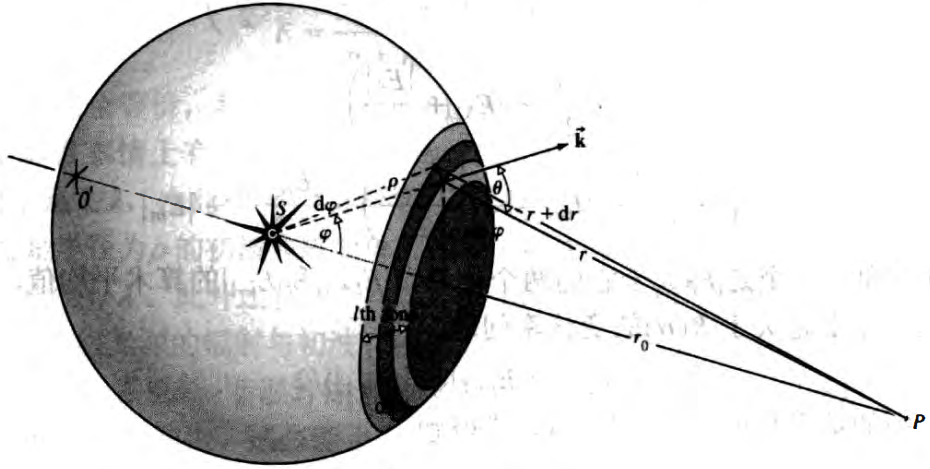
\includegraphics[width=0.6\columnwidth]{assets/4/4.5 球形波阵面的传播.png}
    \caption{球形波阵面的传播}\label{球形波阵面的传播}
\end{figure}

\subsection{圆孔近场衍射}

我们指出,虽然在数学上将半波带分为了无限多个,但由于倾斜因子 $K(\theta)$ 的存在,认为小孔中只能“看到”有限个半波带是合适的。通过计算给定小孔上的半波带数目 $N_F$,可以得到中轴线上辐照度的一个良好近似。每个半波带的面积 $A$ 由下式给出:
\begin{equation}
A = \pi \frac{r_0 \rho}{r_0 + \rho} \lambda \approx \pi r_0 \lambda
\end{equation}
对圆形小孔,半波带数目为:
\begin{equation}
N_F = \frac{\pi a^2}{A} = \frac{(\rho_0 + r_0)a^2 }{r_0 \rho_0 \lambda} \approx \frac{a^2}{ r_0 \lambda}
\end{equation}
上式中 $\rho$ 和 $r_0$ 分别是小孔到光源和观察点的距离,$a$ 是小孔的半径。$N_F$ 常称为菲涅耳数。保持小孔半径不变,当点 $P$ 从无穷远处向小孔靠近时,$r_0$ 由无穷到 0,$N_F$ 会由 $0$ 逐渐增大为 $\infty$。

由图 \ref{振动曲线} (c) 可以看出在不同半波带数目下,中轴线上的振幅情况。角度还可看出,实际相位角与惠更斯-菲涅尔原理所预测的相位角的不同,$O_s$ 点的切线(向右)是惠更斯-菲涅尔原理的相位角,而相矢量 $\overrightarrow{O_sA_s}$ 的切线对应实际相位角。

\begin{figure}[H]\centering
\begin{subfigure}[b]{0.33\columnwidth}\centering
    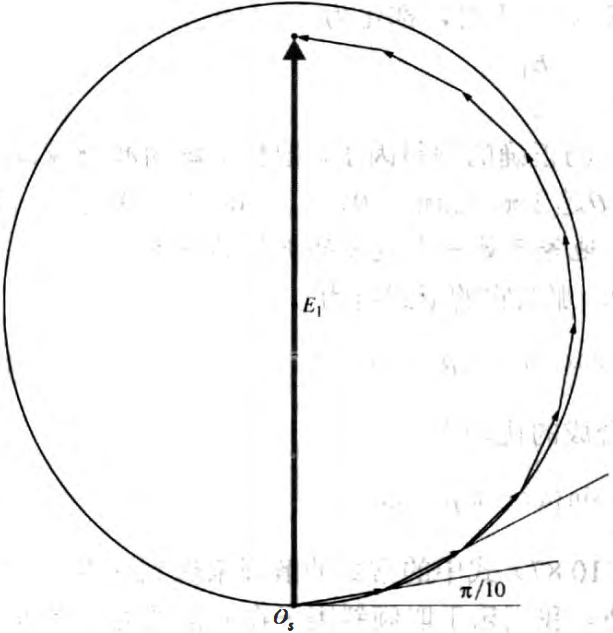
\includegraphics[height=130pt]{assets/4/4.5 相矢量叠加.png}
    \caption{相矢量叠加}
\end{subfigure}
\begin{subfigure}[b]{0.33\columnwidth}\centering
    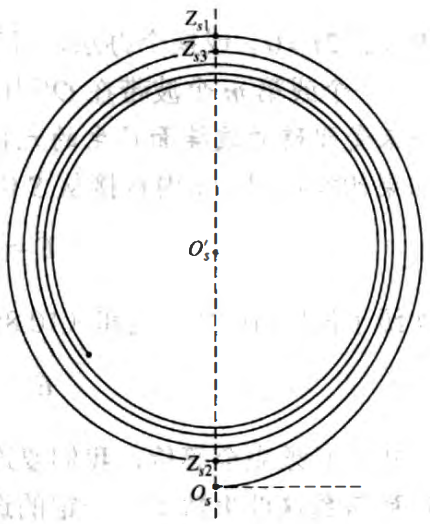
\includegraphics[height=130pt]{assets/4/4.5 总振幅随波带数目的变化.png}
    \caption{总振幅随波带数目的变化}
\end{subfigure}
\begin{subfigure}[b]{0.33\columnwidth}\centering
    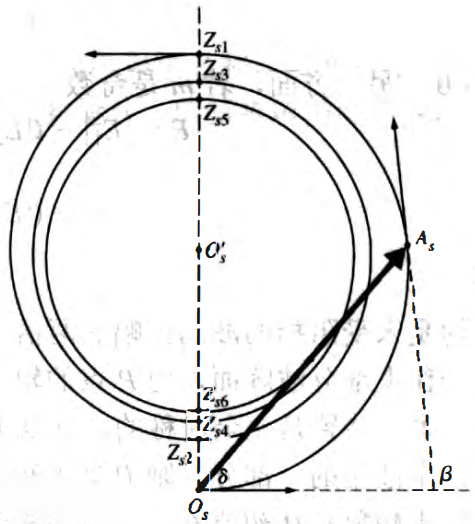
\includegraphics[height=130pt]{assets/4/4.5 振动曲线.png}
    \caption{振动曲线}
\end{subfigure}
\caption{利用波带和振动曲线来判断中轴线上的振幅情况}
\label{振动曲线}
\end{figure}

在固定直径的孔内,由于 $A = \frac{\pi a^2}{N_F}$,随着 $N_F$ 的增大,每个波带的面积 $A$ 会减小,使得轴上辐照度的极大值将依 $\frac{1}{N_F^2}$ 减小(包络线)。一个定性的近似是 $I = I(0) \sinc^2 \left(\frac{\pi}{2}N_F\right)$,其中 $I(0)$ 是 $N_F = 0$ ($P$ 点离小孔无穷远),作出 $I$ 关于 $N_F$ 的变化情况,如图 \ref{中心振幅随波带数的变化} 所示:

\begin{figure}[H]\centering
\begin{subfigure}[b]{0.5\columnwidth}\centering
    \includegraphics[height=185pt]{assets/4/4.5 中心振幅随波带数的变化 2.pdf}
    \caption{$N_F \in [0, 10]$}
\end{subfigure}\hfill
\begin{subfigure}[b]{0.5\columnwidth}\centering
    \includegraphics[height=185pt]{assets/4/4.5 中心振幅随波带数的变化.pdf}
    \caption{$N_F \in [0, 4]$}
\end{subfigure}
\caption{中心振幅随波带数的变化}
\label{中心振幅随波带数的变化}
\end{figure}


另外,当观察点不在中轴线上时,随着点 $P$ 向外移动,“观察”到的波带也会发生变化,如图 \ref{圆孔向外移动},此时辐照度会有一系列极大与极小值,变化比较复杂。对整个观察平面而言,所得衍射图样随着 $N_F$ 的变化而变化,如图 \ref{不同菲涅尔数时的圆孔衍射图样} 所示。
\begin{figure}[H]\centering
    \includegraphics[width=0.75\columnwidth]{assets/4/4.5 圆孔向外移动.png}
    \caption{圆孔内“观察”到的波带}\label{圆孔向外移动}
\end{figure}
\begin{figure}[H]\centering
\begin{subfigure}[b]{0.59\columnwidth}\centering
    \includegraphics[height=185pt]{assets/4/4.5 菲涅尔衍射 不同波带 1.png}
\end{subfigure}
\begin{subfigure}[b]{0.39\columnwidth}\centering
    \includegraphics[height=185pt]{assets/4/4.5 菲涅尔衍射 不同波带.png}
\end{subfigure}
\caption{不同菲涅尔数 $N_F$ 时的圆孔衍射图样}
\label{不同菲涅尔数时的圆孔衍射图样}
\end{figure}



可以看到,当 $N_F \to 0 $ 时(即 $N_F \gg 1$),发生夫琅禾费衍射,这实质上是夫琅禾费衍射的另一种判别方法;当 $N_F \geqslant 1$ 时,发生菲涅尔衍射。特别地,对于环形孔,我们也可以借助振动曲线来分析,如下图:
\begin{figure}[H]\centering
    \includegraphics[width=0.65\columnwidth]{assets/4/4.5 菲涅尔圆环的轴上振幅.png}
    \caption{透光圆环中心轴上的菲涅尔衍射情况}\label{透光圆环中心轴上的菲涅尔衍射情况}
\end{figure}
图 \ref{透光圆环中心轴上的菲涅尔衍射情况} 是一个包含 $\frac{1}{3} + 3 + \frac{1}{3}$ 个波带的环形孔,中心波带(第一波带)被圆盘挡住大约 $\frac{2}{3}$(剩余 $\frac{1}{3}$),振动曲线的 $A_s$ 和 $B_s$ 分别对应图中 $A$ 点和 $B$ 点。由合成结果知道,相矢量 $\overrightarrow{A_sB_s}$ 给出了振幅的大小和相位。

\subsection{圆盘近场衍射}

我们知道,一个未受阻碍的波有无穷多个波带到达 $P$ 点(中轴线上一点),在此处产生一个大小约为第一波带一半的电场,即 $E \approx \frac{1}{2} E_1$。如果障碍物正好盖住第一波带,在振动曲线中减去第一波带的贡献,此时的电场 $E' = -\frac{1}{2}E_1$,这表明障碍物的加入不会改变点 $P$ 的亮暗状态(仍是亮斑)。

用类似的思想,如果障碍物从无开始,逐渐遮住 $1, 2, ..., n$ 个波带,这相当于对给定的圆屏,点 $P$ 由无穷远向圆盘靠近。由振动曲线可看出,除非 $n$ 非常大($P$ 离圆盘很近),相矢量 $\overrightarrow{A_sB_s}$ 的振幅始终不(近似)为 0。这表明 {\bfseries 除了紧挨着圆盘之后的一小段,中轴线上处处为亮点(辐照度始终不为 0),但可能是(与圆盘平行的)平面上的极小值}。遮住前 $n$ 个波带时的电场可写为:
\begin{equation}
E = \frac{1}{2} E_{n+1} = (-1)^{n} K_{n+1} \frac{\varepsilon_A \rho_0 \lambda}{\rho_0 + r_0} \,e^{i\left(k(\rho_0 + r_0) - \omega t\right)} = (-1)^{n} K_n E_0
\end{equation}
其中 $E_0$ 是无阻挡时的电场,$K_n$ 是第 $n$ 级波带法线与中轴线的夹角,随着 $n$ 的增大,夹角逐渐向 $\pi$ 靠近。放到图 \ref{圆盘障碍物衍射} (b) 中,便是点 $A_s$ 逆时针绕振动不断旋转,随着 $N_F$ 的增大,逐渐向中心点 $O_s'$ 靠近,直到 $A_s$ 和 $O_s'$ 重合,$| E | = 0 $。

\begin{figure}[H]\centering
\begin{subfigure}[b]{0.5\columnwidth}\centering
    \includegraphics[height=160pt]{assets/4/4.5 菲涅尔圆形障碍物.png}
    \caption{直径为 3 mm 滚珠的衍射图样}
\end{subfigure}\hfill
\begin{subfigure}[b]{0.5\columnwidth}\centering
    \includegraphics[height=160pt]{assets/4/4.5 圆盘衍射时的振动曲线.png}
    \caption{圆盘衍射时振动曲线上的相矢量}
\end{subfigure}
\caption{圆盘障碍物衍射}
\label{圆盘障碍物衍射}
\end{figure}



\section{讨论光栅的自由光谱范围。}
光栅方程为:
\begin{equation}
a \left(\sin \theta_m  - \sin \theta_i \right) = m \lambda,\quad m = 0, \pm1, \pm2, ...
\end{equation}
其中 $a$ 是光栅常数,表示两相邻狭缝的间距,即周期长度。以垂直于光栅平面的直线为法线,$\theta_i$ 是入射角而 $\theta_m$ 是第 $m$ 级(极大)衍射角。对于正入射的情况,$\theta_i = 0 \Longrightarrow m < \frac{a}{\lambda}$,对于自准直装置,$\theta_i = -\theta_m \Longleftarrow m < \frac{2a}{\lambda}$。

考虑光栅的自由光谱范围,由于波长小(频率高)的光谱线更密集,当 $\lambda_0 - \frac{\Delta \lambda}{2}$ 的第 $m+1$ 级与 $\lambda_0 + \frac{\Delta \lambda}{2}$ 的第 $m$ 级重合时,达到自由光谱范围 $\left(\Delta \lambda\right)_{\text{fsr}}$ :
\begin{equation}
\begin{cases}
    a(\sin \theta_m - \sin \theta_i ) = (m+1)\left(\lambda_0 - \frac{\Delta \lambda}{2}\right) \\ 
    a(\sin \theta_m - \sin \theta_i ) = m\left(\lambda_0 + \frac{\Delta \lambda}{2}\right)
\end{cases}
\Longrightarrow 
\left(\Delta \lambda\right)_{\text{fsr}} = \frac{\lambda_0}{m}
\end{equation}
上面所有公式中的级数 $m$ 在范围 $[0, \frac{2a}{\lambda})$ 内。由此可得到各参数在不同要求下的最值,这与当初 F-P 时的讨论类似,我们不多赘述。


\section{波长为 634.8 nm 的平行光射向直径为 2.76 mm 的圆孔,与孔相距 1 m 处放一屏。回答下面两个问题:(1) 屏上正对圆孔中心的 $P$ 点是亮点还是暗点?(2) 要使 $P$ 点变成与 (1) 相反的情况,至少要把屏幕分别向前或向后移动多少?}

\subsection{屏上正对圆孔中心的 $P$ 点是亮点还是暗点?}

计算菲涅尔数 $N_F$ : 
\begin{equation}
N_F = \frac{\pi a^2}{A} = \frac{(\rho_0 + r_0) a^2}{r_0 \rho_0 \lambda} \overset{\rho_0 \to \infty}{=} \frac{D^2}{4 r_0 \lambda} = \frac{(2.76 \ \mathrm{mm})^2}{4 \times 1 \ \mathrm{m} \times 634.8 \ \mathrm{nm}} = 3
\end{equation}
$N_F$ 为奇数,因此中心点是亮点。

\subsection{要使 $P$ 点变成与 (1) 相反的情况,至少要把屏幕分别向前或向后移动多少?}

$N_F$ 为偶数时中心成暗点,因此分别令 $N_F$ 为 2 和 4 ,得到:
\begin{equation}
r_0 = \frac{D^2}{4 N_F \lambda} = 1.5 \ \mathrm{m},\quad 0.75 \ \mathrm{m}
\end{equation}
因此至少要把屏幕向 $P$ 点移动 0.25 m,或者把屏幕远离 $P$ 点移动 0.5 m。

\section{一波带片由五个环带组成,第一环带是半径 $0 \sim r_1$ 的不透明圆盘,第二环带半径 $r_1\sim r_2$ 透明,第三环带半径 $r_2\sim r_3$ 不透明,第四环带半径 $r_3\sim r_4$ 透明,第五环带是 $r_4 \sim \infty$ 的不透明区域。用波长 500 nm 的平行单色光照明,最亮的像点在距波带片 1 m 的轴上,试求:(1) $r_1$;(2) 像点的光强;(3) 其它光强极大值出现在轴上的哪些位置?}

\subsection{求 $r_1$}

由题意知主焦距$f = 1 \ \mathrm{m}$ ,因此:
\begin{equation}
f = \frac{R_1^2}{\lambda} \Longrightarrow R_1 = \sqrt{f \lambda} = \sqrt{ 1 \ \mathrm{m} \times 500 \ \mathrm{nm} } = 0.7071 \ \mathrm{mm}
\end{equation}

\subsection{求像点的光强}

像点是第一焦点,波带片如图 \ref{题意中的波带片} 所示。
\begin{figure}[H]\centering
    \includegraphics[width=0.3\columnwidth]{assets/4/波带片.pdf}
    \caption{题意中的波带片}\label{题意中的波带片}
\end{figure}
设没有阻挡时的辐照度为 $I_0$,由于波带片透过第 2 和第 4 个(半)环带,因此振幅和辐照度为:
\begin{equation}
E = 2 E_1 = 4 E_0 \Longrightarrow I = 16 I_0
\end{equation}

\subsection{其它光强极大值出现在轴上的哪些位置?}

\begin{graybox}
\textbf{还是先给出结论,再做详细的讨论:}\\
记主焦点(第一焦点)位于 $r = f_1$ 处,辐照度为 $I_1$,则波带片的所有焦点及其辐照度大小是:
\begin{gather}
    f_1 = \frac{R_1^2}{\lambda},\quad   E_1 \approx n E_0 ,\quad   I_1 \approx n^2 I_0 \\
    f_k = \frac{f_1}{k},\quad I_k = \frac{I_1}{k^2},\quad k = 1, 3, 5, ...
\end{gather}\noindent
\end{graybox}


由图 \ref{波带片} (a),我们先来计算各波带的半径。
\begin{figure}[H]\centering
\begin{subfigure}[b]{0.53\columnwidth}\centering
    \includegraphics[height=160pt]{assets/4/4.5 波带半径计算.png}
    \caption{波带片各级圆环半径的计算}
\end{subfigure}\hfill
\begin{subfigure}[b]{0.46\columnwidth}\centering
    \includegraphics[height=160pt]{assets/4/4.5 波带片次焦点.png}
    \caption{波带片的各级焦点}
\end{subfigure}
\caption{波带片}
\label{波带片}
\end{figure}
将第 $m$ 个波带的外缘标以点 $A_m$,按定义,路程 $S$-$A_m$-$P$ 的光程应当比 $S$-$O$-$P$ 要大 $\frac{m\lambda}{2}$,也即:
\begin{equation}
(\rho_m + r_0) - (\rho_0 + r_0) = m \frac{\lambda}{2}
\end{equation}
作泰勒展开 $\rho_m = \rho_0 + \frac{R_m^2}{2\rho_0}$ 和 $r_m = r_0 + \frac{R_m^2}{2r_0}$,代入得到:
\begin{equation}
R_m = \sqrt{ \frac{m\lambda}{\frac{1}{\rho_0} + \frac{1}{r_0}} } \overset{\rho_0 \to \infty}{=}\sqrt{m r_0 \lambda}
\end{equation}
更精确的公式\footnote{由参考文献 \cite{波带片的设计及其衍射特性研究} Page 3 给出}是 $R_m = \sqrt{mr_0\lambda + \frac{m^2\lambda^2}{4}}$,式中 $\frac{m^2\lambda^2}{4}$ 代表球差。

是上面,我们依据“在点 $r_0$ 的各波带振幅相互加强”的原则,得到了波带片的各级半径,使得点 $P$ 是中轴线上光强最大的一点,此时点 $P$ 称为主焦点或一级焦点,距离 $r_0$ 也相应的记作 $f$ 或 $f_1$,有:
\begin{equation}
f_1 = \frac{R_1^2}{\lambda} \Longrightarrow  \frac{1}{\rho_0} + \frac{1}{r_0} = \frac{1}{f}
\end{equation}
与薄透镜公式有相同的形式,因此,用一光束准直入射给定的波带片(起到 $\rho_0 \to \infty$ 的作业),此时中轴线上最亮的点就是主焦距,它是辐照度分布中的一个极大值(也是最大值),因为在 $f$ 处波带片上的各圆环刚好和波阵面上的各波带重合。

需要注意,上面的“$n$ 级半径”并不是波带片的最大圆环半径,对有 $n_0$ 个圆环的挡光型波带片而言(中心圆算第一个圆环),无穷远处不透光,最外围的第 $n_0$ 级圆环 ($R_{n_0-1} \sim R_{n_0}$) 是透光的,则式中的 $n = n_0$;对透光型波带片而言(如图 \ref{菲涅尔波带片} 所示的正负菲涅尔波带片),无穷远处透光,最外围的第 $n$ 级圆环 ($R_{n_0-1} \sim R_{n_0}$) 是不透光的,因此需要再往外“扩张一个半径”,式中的 $n = n_0 + 1$。当然,实际中的 $n_0$ 一般都较大(100 以上),即使不考虑也几乎没有误差。


为什么我们要说是“一级”焦距?因为波带片本质上还是一个光栅,它(在中轴线上)的衍射图样是一系列的主焦点和次焦点交替出现(次焦点都比主焦点近),如图 \ref{波带片} (b) 所示。下面我们推导这些次焦点的位置和辐照度大小。

只需考虑 $r = \frac{f}{k}, k = 2, 3, 4, ...$ 时的情况,其余情况介于两者中间,可定性地判断辐照度的大小变化,且稍后能轻易知道它们都不是极值点。对于给定的 $k$,点 $P$ 与波带距离 $r = \frac{f}{k}$,我们保持波带片的直径 $D$ 不变,当距离变为原来的 $\frac{1}{k}$,由 $R_m = \sqrt{mr\lambda}$ 知道,$P$ 点“看到”的各波带半径变为原来的 $\frac{1}{\sqrt{k}}$。之前 $r = f$ 时波带片共有 $n$ 个半径,“孔”(波带片)的直径没变,而波带半径缩小为原来的 $\frac{1}{\sqrt{k}}$,因此在点 $P$ “看到” 的波带由 $n$ 个增长至 $kn$ 个。

记 $r = \frac{f}{k}$ 时,$P$ 点“看到”的一系列波带半径为 $R_j^{(k)}$,$k = 1, 2, 3, \ \ j = 1, 2, ..., kn$,将它们的相对大小($\frac{R_j^{(k)}}{R_1^(1)}$)如表 \ref{孔内不同波带的半径及位置关系} 一样列出,一切都会变得显然:
\begin{table}[H]\centering
    %\renewcommand{\arraystretch}{1.5} % 调整行间距为 1.5 倍
    %\setlength{\tabcolsep}{1.5mm} % 调整列间距
    \caption{$r = \frac{f}{k}, k = 1, 2, 3, ... $ 时孔内一系列波带的相对半径及位置关系}
    \label{孔内不同波带的半径及位置关系}
\begin{tabular}{cccccccccc}\toprule
    $k = 1$ & $1$ & $\sqrt{2}$ & $\sqrt{3}$  & ... & $\sqrt{n}$ \\
    \midrule
    $k = 2$ & $(\frac{\sqrt{1}}{\sqrt{2}}, 1)$ & $(\frac{\sqrt{3}}{\sqrt{2}}, 2)$ &  $(\frac{\sqrt{5}}{\sqrt{2}}, \sqrt{3})$  & ... & $(\frac{\sqrt{2n -1 }}{\sqrt{2}}, \sqrt{n})$  \\
    $k = 3$ &  $(\frac{\sqrt{1}}{\sqrt{3}}, \frac{\sqrt{2}}{\sqrt{3}}, 1)$ & $(\frac{\sqrt{4}}{\sqrt{3}}, \frac{\sqrt{5}}{\sqrt{3}}, \sqrt{2})$ &  $(\frac{\sqrt{7}}{\sqrt{3}}, \frac{\sqrt{8}}{\sqrt{3}}, \sqrt{3})$  & ... & $(\frac{\sqrt{3n -1 }}{\sqrt{3}}, \frac{\sqrt{3n-2}}{\sqrt{3}}, \sqrt{n})$   \\
    $k = 4$ &  $(\frac{\sqrt{1}}{\sqrt{4}}, \frac{\sqrt{2}}{\sqrt{4}}, \frac{\sqrt{3}}{\sqrt{4}}, 1)$ & $(\frac{\sqrt{5}}{\sqrt{4}}, \frac{\sqrt{6}}{\sqrt{4}}, \frac{7}{\sqrt{4}}, \sqrt{2})$ &  $(\frac{\sqrt{9}}{\sqrt{4}}, \frac{\sqrt{10}}{\sqrt{4}}, \frac{\sqrt{11}}{\sqrt{4}}, \sqrt{3})$  & ... & $(\frac{\sqrt{4n -1 }}{\sqrt{4}}, \frac{\sqrt{4n-2}}{\sqrt{4}}, \frac{\sqrt{4n-3}}{\sqrt{4}}, \sqrt{n})$   \\
    \bottomrule
\end{tabular}
\end{table}

可以看到,当 $k$ 是奇数时,波带片的一个圆环内透过奇数个相邻波带,抵消之后仍剩一个波带的振幅,呈现亮斑;当 $k$ 是偶数时,波带片的一个圆环内透过偶数个相邻波带,抵消之后剩下的是零振幅,呈现暗斑。因此,波带片的所有焦点位置是 $\frac{f}{1}, \frac{f}{3}, \frac{f}{5}, ...$。

再来看辐照度大小,在 $k$ 为奇数的情况下,每个波带片环相当于只透过一个波带,由 $A = \pi r_0 \lambda$ 知道波带面积缩小为原来的 $\frac{1}{k}$,因此电场振幅变为原来的 $\frac{1}{k}$,辐照度变为原来的 $\frac{1}{k^2}$。综上,波带片的所有焦点和辐照度大小是:
\begin{gather}
f_1 = \frac{R_1^2}{\lambda},\quad   E_1 \approx n E_0 ,\quad   I_1 \approx n^2 I_0 \\
f_k = \frac{f_1}{k},\quad I_k = \frac{I_1}{k^2},\quad k = 1, 3, 5, ...
\end{gather}
式中 $n$ 为波带片最外圆的半径级数,也即波带片圆环总个数,$E_0$ 和 $I_0$ 分别是无阻挡时的振幅和辐照度。

\section{一束波长为 500 nm 的平行光垂直照射在一个单缝上,如果所用的单缝的宽度 $a=0.5 \ \mathrm{mm}$,缝后紧挨着的薄透镜焦距 $f=1$ m ,试求: (1) 中央明条纹的角宽度; (2) 中央亮纹的线宽度; (3) 第一级与第二级暗纹的距离。}

\begin{graybox}
本题中的计算都可以借助近似来完成,但考虑到手边有计算机,我们还是取原公式来精确计算。从计算结果我们也可以看到,在小角近似下的误差是非常小的。
\end{graybox}

\subsection{中央明条纹的角宽度}

计算菲涅尔数 $N_F$ : 
\begin{equation}
N_F = \frac{b^2}{f \lambda} = \frac{(0.5 \ \mathrm{mm})^2}{1 \ \mathrm{m} \times 500 \ \mathrm{nm}} = 0.5
\end{equation}
可以近似认为发生的是夫琅禾费衍射。由夫琅禾费单缝衍射公式:
\begin{equation}
I = I(0) \sinc^2 \beta,\quad \beta = \frac{1}{2}kb \sin \theta
\end{equation}
可以推得全峰角宽度 $\xi_\theta$ : 
\begin{gather}
    I = I(0) \sinc^2 \beta =  I(0) \sinc^2\left( \frac{\pi b}{\lambda} \sin \theta \right) = I(0) \sinc^2\left( N \pi \sin \theta \right) \\ 
    b \sin \theta_0 = \lambda \Longrightarrow \xi_{\theta} = 2 \theta_0 = 2 \arcsin \left(\frac{\lambda}{b}\right) = 2 \arcsin \left(\frac{1}{N}\right)
\end{gather}
代入数据:
\begin{equation}
    \xi_\theta = 2 \arcsin \left( \frac{500 \ \mathrm{nm}}{ 0.5 \ \mathrm{mm} } \right) = 0.00200000033 \ \mathrm{rad} \approx 0.0020 \ \mathrm{rad}
\end{equation}

\subsection{中央亮纹的线宽度}
借助狭缝中心点在屏幕上的成像,可以帮助我们推导辐照度随位置 $z$ 的分布。可以计算中央极大的全峰线宽度 $\xi_z$ : 
\begin{gather}
    \sin \theta_0 = \frac{\lambda}{b} \Longrightarrow \xi_z = 2 f \tan \theta_0 = 2f\frac{\sin \theta}{\sqrt{1 - \sin^2 \theta}} = \frac{2f}{\sqrt{N^2 - 1}},\quad N = \frac{b}{\lambda}
\end{gather}
代入数据:
\begin{equation}
N = \frac{0.5 \ \mathrm{mm}}{0.5 \ \mathrm{\mu m}} = 1000 \Longrightarrow \xi_z = \frac{2 \times 1 \ \mathrm{m}}{\sqrt{1000^2 - 1}} = 0.0020000010 \ \mathrm{m} \approx 2.0 \ \mathrm{mm}
\end{equation}

\subsection{第一级与第二级暗纹的距离}
由单缝夫琅禾费衍射公式,可得极小值(暗斑)对应的角度:
\begin{equation}
b\sin \theta_m = m\lambda \Longrightarrow \sin \theta_m = \frac{m\lambda}{b},\quad m = 1, 2, ...
\end{equation}
于是一级和二级暗斑距离为:
\begin{equation}
\Delta x = f\tan \theta_2 - f \tan \theta_1 = f\left[ \frac{\sin \theta_2}{\sqrt{1 - \sin^2 \theta_2}} - \frac{\sin \theta_1}{\sqrt{1 - \sin^2 \theta_1}} \right],\quad \sin \theta_1 = \frac{\lambda}{b},\ \sin \theta_2 = \frac{2\lambda}{b}
\end{equation}
代入数据:
\begin{equation}
    \Delta x = 0.00100000350 \ \mathrm{m} \approx 1.0 \ \mathrm{mm}
\end{equation}

\section{一束白光垂直照射在一光栅上,在形成的同一级光栅光谱中,偏离中央明纹最远的是红光还是蓝光?为什么?}
\vspace*{-3mm}
由单缝夫琅禾费衍射公式,可得极大值(亮斑)对应的角度:
\begin{equation}
b\sin \theta_m = \left(m + \frac{1}{2}\right)\lambda,\quad m = 1, 2, ...
\end{equation}
从蓝光到红光,随着 $\lambda$ 的增大,同级下的 $\theta_m$ 也增大,因此红光散射角度更大,偏离中央明纹最远的是红光。

\vspace*{-5mm}
\section{波长为 600 nm 的单色光垂直入射在一光栅上,第二级明纹出现在 $\sin \theta_2 = 0.2$ 处,第 4 级为第一个缺级。求 (1) 光栅上相邻两缝的距离是多少? (2) 狭缝可能的最小宽度是多少? (3) 在该最小宽度下,实际上能观察到的全部明纹数是多少?}

\vspace*{-3.5mm}
\subsection{光栅上相邻两缝的距离是多少?}
要相邻两缝的中心距离,即求光栅常数 $a$。由光栅方程:
\begin{equation}
a(\sin \theta_m - \sin \theta_i) = m\lambda,\quad m = 0, \pm1, \pm2, ... \Longrightarrow a = \frac{2 \lambda}{\sin \theta_2} = 6 \ \mathrm{\mu m}
\end{equation}

\vspace*{-8mm}
\subsection{狭缝可能的最小宽度是多少?}
当光栅是多缝光栅时,可以考虑狭缝宽度的概念。设光栅有 $N_\text{s}$ 条多缝,有多缝夫琅禾费衍射公式:
\begin{equation}
I = I(0) \sinc^2 \beta\  \frac{\sin^2 N_\text{s} \alpha}{N_s^2 \sin^2 \alpha} ,\quad \beta = \frac{1}{2}kb \sin \theta,\ \alpha = \frac{1}{2}ka \sin \theta
\end{equation}
设 $m = \frac{a}{b}$,由于第 4 极大是第一个缺级,因此 $m = 4$,得到:
\begin{equation}
b = \frac{a}{4} = 1.5 \ \mathrm{\mu m}
\end{equation}

当然,$m$ 可以适当的有一些变化范围,我们取 $m \in [3.5, 4.5]$,可以得到:
\begin{equation}
b \in [1.33 \ \mathrm{\mu m}, 1.71 \ \mathrm{\mu m}] \Longrightarrow b_{\min} = 1.3  \ \mathrm{\mu m}
\end{equation}

\vspace*{-6.5mm}
\subsection{在该最小宽度下,实际上能观察到的全部明纹数是多少?}

若 $b = 1.5  \ \mathrm{\mu m}$,此时 $m = 4$,实际能观察到的全部明纹数(主衍射峰内的极大,不包括缺级部分)为 $2m - 1 = 7$ 条。但是在 $b_{\min} = 1.33  \ \mathrm{\mu m}$ 下,$m = 4.5$,不好确定能观察到的明纹数,因此我们直接作出图像:
\begin{figure}[H]\centering
\begin{subfigure}[b]{0.5\columnwidth}\centering
    \includegraphics[height=190pt]{assets/4/2024-11-08_01-24-51.pdf}
    \caption{光栅的衍射图样}
\end{subfigure}\hfill
\begin{subfigure}[b]{0.5\columnwidth}\centering
    \includegraphics[height=190pt]{assets/4/2024-11-08_01-24-54.pdf}
    \caption{光栅的对数衍射图样}
\end{subfigure}\vspace*{-5mm}
\caption{光栅的衍射图样}
\end{figure}
由图可知,$b_{\min} = 1.33  \ \mathrm{\mu m}$ 时 ($m = 4.5$) ,实际上能看到 7 条明纹,分别是 $0, \pm 1, \pm 2, \pm 3$ 级明纹。

\chapter{第五章作业}\thispagestyle{fancy}

\section{画出图中各情形出射光的偏振状态}
如图所示:
\begin{figure}[H]\centering
    \includegraphics[width=0.9\columnwidth]{assets/5/cdd7fa86a220309cfdc9f9d7115afc61_720.png}
    \caption{各情形出射光的偏振状态}
\end{figure}

\section{在一对正交的偏振片之间放一块四分之一波片,以自然光入射,回答下面问题。}
\subsection{转动四分之一波片的光轴方向时,出射光的强度怎样变化?有无消光现象?}
可以用 Jones 矩阵来解决这个问题。不妨设第一个偏振片的透光方向水平,第二个偏振片透光方向竖直,四分之一波片的 e 轴(快轴)与水平 $x$ 轴夹角为 $\phi$。则入射光的 Jones 矢量为 $\boldsymbol{E} = (E_x, E_y) = (1, 0)$,四分之一波片的 Jones 矩阵 $\boldsymbol{A_1}$ 和第二个偏振片的 Jones 矩阵 $\boldsymbol{A_2}$ 分别为:
\begin{gather}
\boldsymbol{A_1} = \boldsymbol{R}^{-1}(\phi)\cdot \boldsymbol{A_1}|_{\alpha = 0} \cdot\boldsymbol{R}(\phi)
= 
\begin{bmatrix}
    \cos \phi & -\sin \phi \\
    \sin \phi & \cos \phi
\end{bmatrix}\cdot
\begin{bmatrix}
    1 & 0 \\
    0 & i
\end{bmatrix}\cdot
\begin{bmatrix}
    \cos \phi & \sin \phi \\
    -\sin \phi & \cos \phi
\end{bmatrix}\\ \Longrightarrow 
\boldsymbol{A_1} = 
\begin{bmatrix}
    \cos^2 \phi + i \sin^2 \phi & \cos \phi \sin \phi (1 - i) \\ 
    \cos \phi \sin \phi (1 - i) & \sin^2 \phi + i \cos^2 \phi
\end{bmatrix}
,\quad 
\boldsymbol{A_2} = 
\begin{bmatrix}
    0 & 0 \\
    0 & 1
\end{bmatrix}
\end{gather}
上式中忽略了 $\boldsymbol{A_1}|_{\alpha = 0}$ 前的系数 $e^{i \frac{\pi}{4}}$,因为它不影响最终光强。光从第一个偏振器射出,依次经过四分之一波片和第二个偏振器,得到出射的 Jones 矢量为:
\begin{gather}
\boldsymbol{E'} = \boldsymbol{A_1} \cdot \boldsymbol{E} 
= 
\begin{bmatrix}
    \cos^2 \phi + i \sin^2 \phi \\ \cos \phi \sin \phi (1 - i)
\end{bmatrix}
\\
\boldsymbol{E''} = \boldsymbol{A_2} \cdot \boldsymbol{E'}
= 
\begin{bmatrix}
    0 \\ 
    \sin \phi \cos \phi (1 - i)
\end{bmatrix}
= \frac{\sqrt{2}}{2}\sin 2 \phi 
\begin{bmatrix}
    0 \\ 
    \frac{1 - i}{\sqrt{2}}
\end{bmatrix}
\end{gather}
设介质的绝对介电常量为 $\varepsilon$,光在其中的速率为 $v$,我们有辐照度 $I$ : 
\begin{equation}
I = \langle S \rangle_T = \varepsilon v  \langle E^2 \rangle_T = 
\frac{1}{2}\varepsilon v E_0^2 = \frac{1}{4}\varepsilon v\, \sin^2 (2 \phi)
\end{equation}
显然,随着波片的转动,$\phi$ 不断变化,光强也在最大值和最小值(消光)之间周期性变化,因此会出现消光现象。


\subsection{如果有强度极大和消光现象,它们在四分之一波片的光轴处于什么方向时出现?这时从四分之一波片射出的光的偏振态如何?}
做出光强随 $\phi$ 变化的图像,如下图所示:
\begin{figure}[H]\centering
    \includegraphics[width=0.95\columnwidth]{assets/5/2024-11-23_23-01-39.pdf}
    \caption{}
\end{figure}
由图可知,当 $\phi = \frac{\pi}{4} + \frac{k\pi}{2}, k \in \Z$ 时,出射光强为极大值,此时出射光为竖直线偏振。当 $\phi = \frac{k\pi}{2}, k \in \Z$ 时,出现消光现象,此时出射光为水平线偏振。

\section{在实验中偏振片和四分之一波片上透振方向和光轴方向都没有标出,而在检验椭圆偏振光的第二步中需要将四分之一波片的光轴对准椭圆的主轴之一。你能设计一个方案,利用两块偏振片和一块四分之一波片做到这一点吗?}
依次放置偏振片 1、四分之一波片和偏振片 2(此时两个偏振片的透光方向未知),不断转动波片使得出射光光强最大,此时波片快轴要么和偏振片 1 的透光方向平行,要么垂直。固定波片不动,再转动偏振片 2 到恰好消光,此时偏振片 2 的透光方向即与偏振片 1 的透光方向垂直。

固定三个器件的相对角度,当椭圆偏振光入射时,同时转动三个仪器,直到出现消光现象,此时四分之一波片的光轴方向即与椭圆的主轴之一平行。


\section{如图入射的线偏振经过二分之一波片后,偏振态如何变化?如果入射的是圆偏振光呢?}
图 \ref{} (a) 中并没有标明是否有 $E_e \geqslant E_o$,但无论 $E_e \geqslant E_o$ 的大小关系如何,入射光通过二分之一波片后,oe 相位增量 $\Delta \phi = \pi$,所以出射光也为线偏振,如图 \ref{} (b) 所示:
\begin{figure}[H]\centering
\begin{subfigure}[b]{0.5\columnwidth}\centering
    \includegraphics[height=150pt]{assets/5/70d03ee8a05a5bd17b046b52226d661e.png}
    \caption{入射光的偏振态}
\end{subfigure}\hfill
\begin{subfigure}[b]{0.5\columnwidth}\centering
    \includegraphics[height=150pt]{assets/5/53f93c5aebbefb3c222b5250b2da2139_720.png}
    \caption{通过二分之一波片后的偏振态}
\end{subfigure}
\caption{线偏振经过二分之一波片}
\end{figure}

\section{两个偏振片中间是冰洲石,两偏振片透振方向互相垂直,冰洲石的光轴方向居于分角线,正入射光波长 589 nm,冰洲石厚度满足什么条件,P2后出射光强最大?($n_o$ = 1.65836, $n_e$ = 1.48541)}
利用矩阵方法可以很轻松地分析这个问题。不妨设第一个偏振片水平,第二个偏振片竖直,则波片倾角 $\phi = \frac{\pi}{4}$。设冰洲石厚度为 $d$,则相位增量 $\Delta \psi = \frac{2\pi}{\lambda} (n_o - n_e) d$,由此写出波片的 Jones 矩阵 $\boldsymbol{A_1}$ :
\begin{gather}
\boldsymbol{A_1}|_{\alpha = 0} = 
\begin{bmatrix}
    e^{i\frac{\Delta \psi}{2}} & 0 \\
    0 & e^{-i\frac{\Delta \psi}{2}}
\end{bmatrix}
,\quad \boldsymbol{A_1} = \boldsymbol{R}^{-1}(\frac{\pi}{4})\cdot \boldsymbol{A_1}|_{\alpha = 0} \cdot\boldsymbol{R}(\frac{\pi}{4})
\\ 
\Longrightarrow 
\boldsymbol{A_1}
= 
\frac{1}{2}
\begin{bmatrix}
    {\mathrm{e}}^{-\frac{\psi \,\mathrm{i}}{2}} +{\mathrm{e}}^{\frac{\psi \,\mathrm{i}}{2}}  & -{\mathrm{e}}^{-\frac{\psi \,\mathrm{i}}{2}} +{\mathrm{e}}^{\frac{\psi \,\mathrm{i}}{2}} \\
    -{\mathrm{e}}^{-\frac{\psi \,\mathrm{i}}{2}} +{\mathrm{e}}^{\frac{\psi \,\mathrm{i}}{2}}  & {\mathrm{e}}^{-\frac{\psi \,\mathrm{i}}{2}} +{\mathrm{e}}^{\frac{\psi \,\mathrm{i}}{2}} 
\end{bmatrix}
\end{gather}
入射光为 $\boldsymbol{E} = (1, 0)$,依次通过 $\boldsymbol{A_1}$、$\boldsymbol{A_2}$ 之后,出射光为:
\begin{equation}
\boldsymbol{E'} = \boldsymbol{A_2} \cdot \boldsymbol{A_1} \cdot \boldsymbol{E} = 
\frac{1}{2}
\begin{bmatrix}
    0 \\
    e^{\frac{\psi i}{2}} - e^{-\frac{\psi i}{2}}
\end{bmatrix}
= 
\begin{bmatrix}
    0 \\ 
    i \sin \frac{\psi}{2}
\end{bmatrix}
\end{equation}
得到出射光强 $I$ :
\begin{equation}
I = \frac{1}{2} \varepsilon v \sin^2 \frac{\psi}{2}
\end{equation}
当且仅当 $\frac{\psi}{2} = \frac{\pi}{2} + k\pi, k \in \Z$ 时,出射光强最大,这等价于:
\begin{equation}
\frac{1}{2}\cdot \frac{2\pi}{\lambda} (n_o - n_e)d = \frac{\pi}{2} + k\pi \Longrightarrow d = \left(\frac{1}{2} + k\right) \cdot \frac{\lambda}{n_o - n_e},\quad k = 0, 1, 2, ...
\end{equation}
写成数值形式,即为:
\begin{equation}
d = (0.5 + k) \cdot 3.4056 \ \mathrm{\mu m} = 1.7028 \ \mathrm{\mu m},\ 5.1084 \ \mathrm{\mu m},\ 8.5140 \ \mathrm{\mu m}, 11.9196 \ \mathrm{\mu m}, ...
\end{equation}

\section{两个偏振片中间是两块冰洲石,两偏振片透振方向互相垂直,两冰洲石的光轴方向垂直,分别位于两个分角线,两冰洲石厚度相等,正入射光波长 589 nm,P2 后出射光强如何?}
与上一题类似,记两个波片的 Jones 矩阵分别为 $\boldsymbol{A_1}$、$\boldsymbol{A_2}$,则有:
\begin{equation}
\boldsymbol{A_1} = \frac{1}{2}
\begin{bmatrix}
    {\mathrm{e}}^{-\frac{\psi \,\mathrm{i}}{2}} +{\mathrm{e}}^{\frac{\psi \,\mathrm{i}}{2}}  & -{\mathrm{e}}^{-\frac{\psi \,\mathrm{i}}{2}} +{\mathrm{e}}^{\frac{\psi \,\mathrm{i}}{2}} \\
    -{\mathrm{e}}^{-\frac{\psi \,\mathrm{i}}{2}} +{\mathrm{e}}^{\frac{\psi \,\mathrm{i}}{2}}  & {\mathrm{e}}^{-\frac{\psi \,\mathrm{i}}{2}} +{\mathrm{e}}^{\frac{\psi \,\mathrm{i}}{2}} 
\end{bmatrix}
,\quad 
\boldsymbol{A_2} = \frac{1}{2}
\begin{bmatrix}
    {\mathrm{e}}^{-\frac{\psi \,\mathrm{i}}{2}} +{\mathrm{e}}^{\frac{\psi \,\mathrm{i}}{2}}  & {\mathrm{e}}^{-\frac{\psi \,\mathrm{i}}{2}} -{\mathrm{e}}^{\frac{\psi \,\mathrm{i}}{2}} \\
    {\mathrm{e}}^{-\frac{\psi \,\mathrm{i}}{2}} -{\mathrm{e}}^{\frac{\psi \,\mathrm{i}}{2}}  & {\mathrm{e}}^{-\frac{\psi \,\mathrm{i}}{2}} +{\mathrm{e}}^{\frac{\psi \,\mathrm{i}}{2}}
\end{bmatrix}
\end{equation}
入射光 $\boldsymbol{E} = (1, 0)$,出射光 $\boldsymbol{E'}$ 为:
\begin{equation}
\boldsymbol{E'} = \boldsymbol{A_3}\boldsymbol{A_2}\boldsymbol{A_1} \boldsymbol{E} = 
\begin{bmatrix}
    0 \\ 
    0
\end{bmatrix}
\end{equation}
这意味着无论冰洲石的厚度如何,出射光强都恒为 0。

\section{已知水晶对 589 nm 的旋光率 $\alpha$ = 21.75$^\circ\cdot \ \mathrm{mm}^{-1}$,求左、右旋圆偏振光折射率之差。}
旋光率 $\alpha$ 满足:
\begin{equation}
\Delta \psi = \frac{1}{2} \cdot \frac{2\pi}{\lambda}(n_R - n_L) d = \alpha d \Longrightarrow n_R - n_L = \frac{\alpha \lambda}{\pi} = 7.1171 \times 10^{-5}
\end{equation}
即左、右旋圆偏振光折射率之差为 $7.1171 \times 10^{-5}$。

% --------------------------- 附录 --------------------------- %
% >> ------------------------ 附录 ------------------------ << %

\newpage
\appendix
% chapter 标题自定义设置
\titleformat{\chapter}[hang]{\normalfont\huge\bfseries\centering}{}{20pt}{}
\titlespacing*{\chapter}{0pt}{-25pt}{8pt} % 控制上方空白的大小
% section 标题自定义设置 
\titleformat{\section}[hang]{\normalfont\centering\Large\bfseries}{\thesection}{8pt}{}
\lhead{附录 \thechapter}

% 附录 A
\chapter*{附录 A\hspace*{20pt}  Matlab 代码}\setcounter{chapter}{1} 
\setcounter{equation}{0}    % 重置公式计数器   
\addcontentsline{toc}{chapter}{附录 A\hspace*{6pt}  Matlab 代码}   
\thispagestyle{fancy} 
\setcounter{section}{0}   
\renewcommand\thesection{A.\arabic{section}}   
\renewcommand{\thefigure}{A.\arabic{figure}} 
\renewcommand{\thetable}{A.\arabic{table}}


\section{图 \ref{振幅系数随入射角的变化} 源码}\label{图振幅系数随入射角的变化源码}
\begin{matlablisting}
%%%%%%%%%% 空气入射玻璃 %%%%%%%%%%
global n_i n_t
n_i = 1;
n_t = 1.5;

theta_t = @(theta_i) asin(n_i/n_t*sin(theta_i));
r_s = @(theta_i, theta_t) - sin(theta_i - theta_t)./sin(theta_i + theta_t);
r_p = @(theta_i, theta_t) + tan(theta_i - theta_t)./tan(theta_i + theta_t);
t_s = @(theta_i, theta_t) 2*sin(theta_t).*cos(theta_i)./sin(theta_i + theta_t);
t_p = @(theta_i, theta_t) 2*sin(theta_t).*cos(theta_i) ./ ( sin(theta_i + theta_t).*cos(theta_i - theta_t) );
theta_B = atan(n_t/n_i);
theta_C = asin(n_t/n_i);

theta_array = linspace(-0.1, pi/2, 101);
Y = [
    r_s(theta_array, theta_t(theta_array))
    r_p(theta_array, theta_t(theta_array))
    t_s(theta_array, theta_t(theta_array))
    t_p(theta_array, theta_t(theta_array))
    ];
stc = MyPlot(theta_array, Y);
xline(theta_B, 'b')
yline(0)
xlim([0, pi/2])
ylim([-1, 1])
stc.leg.String = ["$r_s$"; "$r_p$"; "$t_s$"; "$t_p$"; "$\theta_i = \theta_B$"];
stc.leg.Interpreter = "latex";
stc.leg.FontSize = 14;
stc.leg.Location = "southwest";
stc.axes.Title.String = '$n_i = 1 < n_t = 1.5$';
stc.axes.Title.Interpreter = "latex";
stc.label.x.String = '$\theta_i$';
stc.label.y.String = '$r$';
stc.plot.plot_3.LineStyle = ":";
stc.plot.plot_3.Color = 'b';
stc.plot.plot_4.LineStyle = ":";
stc.plot.plot_4.Color = [1 0 1];
%MyExport_pdf

%%%%%%%%%% 玻璃入射空气 %%%%%%%%%%
n_i = 1.5;
n_t = 1;

theta_t = @(theta_i) asin(n_i/n_t*sin(theta_i));
r_s = @(theta_i, theta_t) - sin(theta_i - theta_t)./sin(theta_i + theta_t);
r_p = @(theta_i, theta_t) + tan(theta_i - theta_t)./tan(theta_i + theta_t);
t_s = @(theta_i, theta_t) 2*sin(theta_t).*cos(theta_i)./sin(theta_i + theta_t);
t_p = @(theta_i, theta_t) 2*sin(theta_t).*cos(theta_i) ./ ( sin(theta_i + theta_t).*cos(theta_i - theta_t) );
theta_B = atan(n_t/n_i);
theta_C = asin(n_t/n_i);


theta_array = linspace(0, theta_C, 101);
Y = [
    r_s(theta_array, theta_t(theta_array))
    r_p(theta_array, theta_t(theta_array))
    t_s(theta_array, theta_t(theta_array))
    t_p(theta_array, theta_t(theta_array))
    ];
stc = MyPlot(theta_array, Y);
xline(theta_B, 'b')
xline(theta_C, 'r')
yline(0)
xlim([0, pi/2])
ylim([-0.5, 3])
stc.leg.String = ["$r_s$"; "$r_p$"; "$t_s$"; "$t_p$"; "$\theta_i = \theta_B$"; "$\theta_i = \theta_C$"];
stc.leg.Interpreter = "latex";
stc.axes.Title.String = '$n_i = 1.5 > n_t = 1$';
stc.axes.Title.Interpreter = "latex";
stc.label.x.String = '$\theta_i$';
stc.label.y.String = '$r$';
stc.plot.plot_3.LineStyle = ":";
stc.plot.plot_3.Color = 'b';
stc.plot.plot_4.LineStyle = ":";
stc.plot.plot_4.Color = [1 0 1];
%MyExport_pdf
\end{matlablisting}

\section{公式 \ref{玻璃折射率} 源码}\label{玻璃折射率源码}

\begin{matlablisting}
R_s = @(n_ti, t) ( (cos(t) - sqrt(n_ti^2 - sin(t)^2)) / (cos(t) + sqrt(n_ti^2 - sin(t)^2)) )^2;
R_p = @(n_ti, t) ( (n_ti^2*cos(t) - sqrt(n_ti^2 - sin(t)^2)) / (n_ti^2*cos(t) + sqrt(n_ti^2 - sin(t)^2)) )^2;

theta_B = @(n_ti) atan(n_ti);
n_ti = fzero(@(n_ti) 0.5*(R_s(n_ti, theta_B(n_ti)) + R_p(n_ti, theta_B(n_ti))) - 0.14, 1);

theta_C = @(n_ti) asin(n_ti);
theta_B = @(n_ti) atan(n_ti);
theta_t = @(n_ti, theta_i) asin(sin(theta_i)/n_ti);

disp(['n_ti = ', num2str(n_ti, '%.6f')])
disp(['theta_i = theta_B = ', num2str(theta_B(n_ti), '%.6f') ' rad = ', num2str(rad2deg(theta_B(n_ti)), '%.6f'), ' deg'])
disp(['theta_t = ', num2str(theta_t(n_ti, theta_B(n_ti)), '%.6f') ' rad = ', num2str(rad2deg(theta_t(n_ti, theta_B(n_ti))), '%.6f'), ' deg'])
disp(['theta_C = ', num2str(theta_C(n_ti), '%.6f') ' rad = ', num2str(rad2deg(theta_C(n_ti)), '%.6f'), ' deg'])
disp(['R_s = ', num2str(R_s(n_ti, theta_B(n_ti)), '%.6f')])
disp(['R_p = ', num2str(R_p(n_ti, theta_B(n_ti)), '%.6f')])
disp(['T_s = ', num2str(1 - R_s(n_ti, theta_B(n_ti)), '%.6f')])
disp(['T_p = ', num2str(1 - R_p(n_ti, theta_B(n_ti)), '%.6f')])
disp(['R = ', num2str( 0.5*(R_s(n_ti, theta_B(n_ti)) + R_p(n_ti, theta_B(n_ti))) , '%.6f')])
disp(['T = ', num2str( 0.5*(2 - R_s(n_ti, theta_B(n_ti)) - R_p(n_ti, theta_B(n_ti))), '%.6f')])


%{
>> Output:
n_ti = 0.554902
theta_i = theta_B = 0.506599 rad = 29.025970 deg
theta_t = 1.064198 rad = 60.974030 deg
theta_C = 0.588245 rad = 33.703947 deg
R_s = 0.280000
R_p = 0.000000
T_s = 0.720000
T_p = 1.000000
R = 0.140000
T = 0.860000
%}
\end{matlablisting}

\section{公式 \ref{解入射角} 源码}\label{公式解入射角源码}

\begin{matlablisting}
R_s = @(n_ti, t) ( (cos(t) - sqrt(n_ti^2 - sin(t)^2)) / (cos(t) + sqrt(n_ti^2 - sin(t)^2)) )^2;
R_p = @(n_ti, t) ( (n_ti^2*cos(t) - sqrt(n_ti^2 - sin(t)^2)) / (n_ti^2*cos(t) + sqrt(n_ti^2 - sin(t)^2)) )^2;

theta_i = fzero(@(t) ( R_s(1.5, t) + R_p(1.5, t) - 2*0.14) , deg2rad(45));
disp(['theta_i = ', num2str(theta_i, '%.6f'), ' rad'])
disp(['theta_i = ', num2str(rad2deg(theta_i), '%.6f'), ' deg'])
disp(['R_s = ', num2str(R_s(1.5, theta_i), '%.6f')])
disp(['R_p = ', num2str(R_p(1.5, theta_i), '%.6f')])
disp(['T_s = ', num2str(1 - R_s(1.5, theta_i), '%.6f')])
disp(['T_p = ', num2str(1 - R_p(1.5, theta_i), '%.6f')])
disp(['R = ', num2str( 0.5*(R_s(1.5, theta_i) + R_p(1.5, theta_i)) , '%.6f')])
disp(['T = ', num2str( 0.5*(2 - R_s(1.5, theta_i) - R_p(1.5, theta_i)), '%.6f')])

%{
>> Output:
theta_i = 1.173220 rad
theta_i = 67.220559 deg
R_s = 0.256933
R_p = 0.023067
T_s = 0.743067
T_p = 0.976933
R = 0.140000
T = 0.860000
%}
\end{matlablisting}

\section{图 \ref{方程左边的变化情况} 源码}\label{方程左边的变化情况源码}

\begin{matlablisting}
R_s = @(n_ti, t) ( (cos(t) - sqrt(n_ti^2 - sin(t)^2)) / (cos(t) + sqrt(n_ti^2 - sin(t)^2)) )^2;
R_p = @(n_ti, t) ( (n_ti^2*cos(t) - sqrt(n_ti^2 - sin(t)^2)) / (n_ti^2*cos(t) + sqrt(n_ti^2 - sin(t)^2)) )^2;
theta_B = @(n_ti) atan(n_ti);

eq_left = @(n_ti) 0.5*(R_s(n_ti, theta_B(n_ti)) + R_p(n_ti, theta_B(n_ti)))

X = linspace(0, 2, 100);
Y = zeros(size(X));
for i = 1:length(X)
    Y(i) = eq_left(X(i));
end

stc = MyPlot(X, Y);
yline(0.14, 'Color', 'r', 'LineWidth', 0.4);
xline(0.554902, 'Color', [0.1, 0.1, 0.1], 'LineWidth', 0.4)
xline(1.802121, 'Color', [0.3, 0.3, 0.3], 'LineWidth', 0.4)
stc.axes.Title.String = '';
stc.label.x.String = '$n_{ti}$';
stc.leg.Location = 'northeast';
hold on
scatter([0.554902, 1.802121], [0.14, 0.14], 180, '.r')
stc.leg.String = ["$y =  0.5\left[ R_s(n_{ti}) + R_p(n_{ti}) \right]$"; "$y = 0.14$"; "$n_{ti} = 0.554902$"; "$n_{ti} = 1.802121$"];
%MyExport_pdf
\end{matlablisting}

% >> ------------------------ 附录 ------------------------ << %
% --------------------------- 附录 --------------------------- %


\end{document}

% VScode 常用快捷键:

% Ctrl + R:                 打开最近的文件夹
% F2:                       变量重命名
% Ctrl + Enter:             行中换行
% Alt + up/down:            上下移行
% 鼠标中键 + 移动:           快速多光标
% Shift + Alt + up/down:    上下复制
% Ctrl + left/right:        左右跳单词
% Ctrl + Backspace/Delete:  左右删单词    
% Shift + Delete:           删除此行
% Ctrl + J:                 打开 VScode 下栏(输出栏)
% Ctrl + B:                 打开 VScode 左栏(目录栏)
% Ctrl + `:                 打开 VScode 终端栏
% Ctrl + 0:                 定位文件
% Ctrl + Tab:               切换已打开的文件(切标签)
% Ctrl + Shift + P:         打开全局命令(设置)

% Latex 常用快捷键

% Ctrl + Alt + J:           由代码定位到PDF
% 


% Git提交规范:
% update: Linear Algebra 2 notes
% add: Linear Algebra 2 notes
% import: Linear Algebra 2 notes
% delete: Linear Algebra 2 notes
